%% bare_conf.tex
%% V1.4b
%% 2015/08/26
%% by Michael Shell
%% See:
%% http://www.michaelshell.org/
%% for current contact information.
%%
%% This is a skeleton file demonstrating the use of IEEEtran.cls
%% (requires IEEEtran.cls version 1.8b or later) with an IEEE
%% conference paper.
%%
%% Support sites:
%% http://www.michaelshell.org/tex/ieeetran/
%% http://www.ctan.org/pkg/ieeetran
%% and
%% http://www.ieee.org/

%%*************************************************************************
%% Legal Notice:
%% This code is offered as-is without any warranty either expressed or
%% implied; without even the implied warranty of MERCHANTABILITY or
%% FITNESS FOR A PARTICULAR PURPOSE! 
%% User assumes all risk.
%% In no event shall the IEEE or any contributor to this code be liable for
%% any damages or losses, including, but not limited to, incidental,
%% consequential, or any other damages, resulting from the use or misuse
%% of any information contained here.
%%
%% All comments are the opinions of their respective authors and are not
%% necessarily endorsed by the IEEE.
%%
%% This work is distributed under the LaTeX Project Public License (LPPL)
%% ( http://www.latex-project.org/ ) version 1.3, and may be freely used,
%% distributed and modified. A copy of the LPPL, version 1.3, is included
%% in the base LaTeX documentation of all distributions of LaTeX released
%% 2003/12/01 or later.
%% Retain all contribution notices and credits.
%% ** Modified files should be clearly indicated as such, including  **
%% ** renaming them and changing author support contact information. **
%%*************************************************************************


% *** Authors should verify (and, if needed, correct) their LaTeX system  ***
% *** with the testflow diagnostic prior to trusting their LaTeX platform ***
% *** with production work. The IEEE's font choices and paper sizes can   ***
% *** trigger bugs that do not appear when using other class files.       ***                          ***
% The testflow support page is at:
% http://www.michaelshell.org/tex/testflow/




\documentclass[conference]{IEEEtran}
% Some Computer Society conferences also require the compsoc mode option,
% but others use the standard conference format.
%
% If IEEEtran.cls has not been installed into the LaTeX system files,
% manually specify the path to it like:
% \documentclass[conference]{../sty/IEEEtran}






% Some very useful LaTeX packages include:
% (uncomment the ones you want to load)


% *** MISC UTILITY PACKAGES ***
%
%\usepackage{ifpdf}
% Heiko Oberdiek's ifpdf.sty is very useful if you need conditional
% compilation based on whether the output is pdf or dvi.
% usage:
% \ifpdf
%   % pdf code
% \else
%   % dvi code
% \fi
% The latest version of ifpdf.sty can be obtained from:
% http://www.ctan.org/pkg/ifpdf
% Also, note that IEEEtran.cls V1.7 and later provides a builtin
% \ifCLASSINFOpdf conditional that works the same way.
% When switching from latex to pdflatex and vice-versa, the compiler may
% have to be run twice to clear warning/error messages.






% *** CITATION PACKAGES ***
%
%\usepackage{cite}
% cite.sty was written by Donald Arseneau
% V1.6 and later of IEEEtran pre-defines the format of the cite.sty package
% \cite{} output to follow that of the IEEE. Loading the cite package will
% result in citation numbers being automatically sorted and properly
% "compressed/ranged". e.g., [1], [9], [2], [7], [5], [6] without using
% cite.sty will become [1], [2], [5]--[7], [9] using cite.sty. cite.sty's
% \cite will automatically add leading space, if needed. Use cite.sty's
% noadjust option (cite.sty V3.8 and later) if you want to turn this off
% such as if a citation ever needs to be enclosed in parenthesis.
% cite.sty is already installed on most LaTeX systems. Be sure and use
% version 5.0 (2009-03-20) and later if using hyperref.sty.
% The latest version can be obtained at:
% http://www.ctan.org/pkg/cite
% The documentation is contained in the cite.sty file itself.






% *** GRAPHICS RELATED PACKAGES ***
%
\ifCLASSINFOpdf
  % \usepackage[pdftex]{graphicx}
  % declare the path(s) where your graphic files are
  % \graphicspath{{../pdf/}{../jpeg/}}
  % and their extensions so you won't have to specify these with
  % every instance of \includegraphics
  % \DeclareGraphicsExtensions{.pdf,.jpeg,.png}
\else
  % or other class option (dvipsone, dvipdf, if not using dvips). graphicx
  % will default to the driver specified in the system graphics.cfg if no
  % driver is specified.
  % \usepackage[dvips]{graphicx}
  % declare the path(s) where your graphic files are
  % \graphicspath{{../eps/}}
  % and their extensions so you won't have to specify these with
  % every instance of \includegraphics
  % \DeclareGraphicsExtensions{.eps}
\fi
% graphicx was written by David Carlisle and Sebastian Rahtz. It is
% required if you want graphics, photos, etc. graphicx.sty is already
% installed on most LaTeX systems. The latest version and documentation
% can be obtained at: 
% http://www.ctan.org/pkg/graphicx
% Another good source of documentation is "Using Imported Graphics in
% LaTeX2e" by Keith Reckdahl which can be found at:
% http://www.ctan.org/pkg/epslatex
%
% latex, and pdflatex in dvi mode, support graphics in encapsulated
% postscript (.eps) format. pdflatex in pdf mode supports graphics
% in .pdf, .jpeg, .png and .mps (metapost) formats. Users should ensure
% that all non-photo figures use a vector format (.eps, .pdf, .mps) and
% not a bitmapped formats (.jpeg, .png). The IEEE frowns on bitmapped formats
% which can result in "jaggedy"/blurry rendering of lines and letters as
% well as large increases in file sizes.
%
% You can find documentation about the pdfTeX application at:
% http://www.tug.org/applications/pdftex





% *** MATH PACKAGES ***
%
%\usepackage{amsmath}
% A popular package from the American Mathematical Society that provides
% many useful and powerful commands for dealing with mathematics.
%
% Note that the amsmath package sets \interdisplaylinepenalty to 10000
% thus preventing page breaks from occurring within multiline equations. Use:
%\interdisplaylinepenalty=2500
% after loading amsmath to restore such page breaks as IEEEtran.cls normally
% does. amsmath.sty is already installed on most LaTeX systems. The latest
% version and documentation can be obtained at:
% http://www.ctan.org/pkg/amsmath





% *** SPECIALIZED LIST PACKAGES ***
%
%\usepackage{algorithmic}
% algorithmic.sty was written by Peter Williams and Rogerio Brito.
% This package provides an algorithmic environment fo describing algorithms.
% You can use the algorithmic environment in-text or within a figure
% environment to provide for a floating algorithm. Do NOT use the algorithm
% floating environment provided by algorithm.sty (by the same authors) or
% algorithm2e.sty (by Christophe Fiorio) as the IEEE does not use dedicated
% algorithm float types and packages that provide these will not provide
% correct IEEE style captions. The latest version and documentation of
% algorithmic.sty can be obtained at:
% http://www.ctan.org/pkg/algorithms
% Also of interest may be the (relatively newer and more customizable)
% algorithmicx.sty package by Szasz Janos:
% http://www.ctan.org/pkg/algorithmicx




% *** ALIGNMENT PACKAGES ***
%
%\usepackage{array}
% Frank Mittelbach's and David Carlisle's array.sty patches and improves
% the standard LaTeX2e array and tabular environments to provide better
% appearance and additional user controls. As the default LaTeX2e table
% generation code is lacking to the point of almost being broken with
% respect to the quality of the end results, all users are strongly
% advised to use an enhanced (at the very least that provided by array.sty)
% set of table tools. array.sty is already installed on most systems. The
% latest version and documentation can be obtained at:
% http://www.ctan.org/pkg/array


% IEEEtran contains the IEEEeqnarray family of commands that can be used to
% generate multiline equations as well as matrices, tables, etc., of high
% quality.




% *** SUBFIGURE PACKAGES ***
%\ifCLASSOPTIONcompsoc
%  \usepackage[caption=false,font=normalsize,labelfont=sf,textfont=sf]{subfig}
%\else
%  \usepackage[caption=false,font=footnotesize]{subfig}
%\fi
% subfig.sty, written by Steven Douglas Cochran, is the modern replacement
% for subfigure.sty, the latter of which is no longer maintained and is
% incompatible with some LaTeX packages including fixltx2e. However,
% subfig.sty requires and automatically loads Axel Sommerfeldt's caption.sty
% which will override IEEEtran.cls' handling of captions and this will result
% in non-IEEE style figure/table captions. To prevent this problem, be sure
% and invoke subfig.sty's "caption=false" package option (available since
% subfig.sty version 1.3, 2005/06/28) as this is will preserve IEEEtran.cls
% handling of captions.
% Note that the Computer Society format requires a larger sans serif font
% than the serif footnote size font used in traditional IEEE formatting
% and thus the need to invoke different subfig.sty package options depending
% on whether compsoc mode has been enabled.
%
% The latest version and documentation of subfig.sty can be obtained at:
% http://www.ctan.org/pkg/subfig




% *** FLOAT PACKAGES ***
%
%\usepackage{fixltx2e}
% fixltx2e, the successor to the earlier fix2col.sty, was written by
% Frank Mittelbach and David Carlisle. This package corrects a few problems
% in the LaTeX2e kernel, the most notable of which is that in current
% LaTeX2e releases, the ordering of single and double column floats is not
% guaranteed to be preserved. Thus, an unpatched LaTeX2e can allow a
% single column figure to be placed prior to an earlier double column
% figure.
% Be aware that LaTeX2e kernels dated 2015 and later have fixltx2e.sty's
% corrections already built into the system in which case a warning will
% be issued if an attempt is made to load fixltx2e.sty as it is no longer
% needed.
% The latest version and documentation can be found at:
% http://www.ctan.org/pkg/fixltx2e


%\usepackage{stfloats}
% stfloats.sty was written by Sigitas Tolusis. This package gives LaTeX2e
% the ability to do double column floats at the bottom of the page as well
% as the top. (e.g., "\begin{figure*}[!b]" is not normally possible in
% LaTeX2e). It also provides a command:
%\fnbelowfloat
% to enable the placement of footnotes below bottom floats (the standard
% LaTeX2e kernel puts them above bottom floats). This is an invasive package
% which rewrites many portions of the LaTeX2e float routines. It may not work
% with other packages that modify the LaTeX2e float routines. The latest
% version and documentation can be obtained at:
% http://www.ctan.org/pkg/stfloats
% Do not use the stfloats baselinefloat ability as the IEEE does not allow
% \baselineskip to stretch. Authors submitting work to the IEEE should note
% that the IEEE rarely uses double column equations and that authors should try
% to avoid such use. Do not be tempted to use the cuted.sty or midfloat.sty
% packages (also by Sigitas Tolusis) as the IEEE does not format its papers in
% such ways.
% Do not attempt to use stfloats with fixltx2e as they are incompatible.
% Instead, use Morten Hogholm'a dblfloatfix which combines the features
% of both fixltx2e and stfloats:
%
% \usepackage{dblfloatfix}
% The latest version can be found at:
% http://www.ctan.org/pkg/dblfloatfix




% *** PDF, URL AND HYPERLINK PACKAGES ***
%
%\usepackage{url}
% url.sty was written by Donald Arseneau. It provides better support for
% handling and breaking URLs. url.sty is already installed on most LaTeX
% systems. The latest version and documentation can be obtained at:
% http://www.ctan.org/pkg/url
% Basically, \url{my_url_here}.




% *** Do not adjust lengths that control margins, column widths, etc. ***
% *** Do not use packages that alter fonts (such as pslatex).         ***
% There should be no need to do such things with IEEEtran.cls V1.6 and later.
% (Unless specifically asked to do so by the journal or conference you plan
% to submit to, of course. )
\usepackage{amsmath,amssymb,amsfonts}
\usepackage{graphicx}
\usepackage{xcolor}
% \usepackage{algorithm}
% \usepackage{algpseudocode}
\usepackage{float}
\usepackage{multirow,enumitem}
\usepackage{appendix}
\usepackage{subcaption}
\usepackage{graphicx}
\usepackage{float}
\usepackage{listings}
\usepackage{algorithmic}
\usepackage{textcomp}
\usepackage{datatool,booktabs}
\usepackage{tabularray}
\usepackage{changepage}
\usepackage{tabularx}
\usepackage{tikz}
\usetikzlibrary{shapes.geometric}
\usepackage{verbatim}

\newcommand{\circled}[1]{\tikz[baseline=(char.base)]{
    \node[shape=circle,fill=white,text=black,draw=black,inner sep=1pt] (char) {#1};}}

\newcommand{\circledw}[1]{\tikz[baseline=(char.base)]{
    \node[shape=circle,fill=white,text=black,draw=black,inner sep=1pt] (char) {#1};}}

\newcommand{\triyellow}{\tikz[baseline=-0.3ex]{
    \node[regular polygon, regular polygon sides=3, fill=yellow,
          draw=black, inner sep=1.5pt, minimum size=0.8em] {};}}

\newcommand{\trigreen}{\tikz[baseline=-0.3ex]{
    \node[regular polygon, regular polygon sides=3, fill=green,
          draw=black, inner sep=1.5pt, minimum size=0.8em] {};}}

\newcommand{\trired}{\tikz[baseline=-0.3ex]{
    \node[regular polygon, regular polygon sides=3, fill=red,
          draw=black, inner sep=1.5pt, minimum size=0.8em] {};}}

\definecolor{bestperf}{HTML}{FF0000} % Navy Blue
% correct bad hyphenation here
\hyphenation{op-tical net-works semi-conduc-tor}

\newcommand{\yash}[1]{\textcolor{red}{[YASH: #1]}}
\newcommand{\todo}[1]{\textcolor{red}{[todo:#1]}}
\newcommand{\lan}[1]{\textcolor{blue}{[LAN:#1]}}
\newcommand{\jor}[1]{\textcolor{green}{[jor:#1]}}
\begin{document}
%
% paper title
% Titles are generally capitalized except for words such as a, an, and, as,
% at, but, by, for, in, nor, of, on, or, the, to and up, which are usually
% not capitalized unless they are the first or last word of the title.
% Linebreaks \\ can be used within to get better formatting as desired.
% Do not put math or special symbols in the title.
\title{MARS: Monte Carlo Tree Search based Adaptive and Responsive Scheduling}


% author names and affiliations
% use a multiple column layout for up to three different
% affiliations
% \author{\IEEEauthorblockN{Michael Shell}
% \IEEEauthorblockA{School of Electrical and\\Computer Engineering\\
% Georgia Institute of Technology\\
% Atlanta, Georgia 30332--0250\\
% Email: http://www.michaelshell.org/contact.html}
% \and
% \IEEEauthorblockN{Homer Simpson}
% \IEEEauthorblockA{Twentieth Century Fox\\
% Springfield, USA\\
% Email: homer@thesimpsons.com}
% \and
% \IEEEauthorblockN{James Kirk\\ and Montgomery Scott}
% \IEEEauthorblockA{Starfleet Academy\\
% San Francisco, California 96678--2391\\
% Telephone: (800) 555--1212\\
% Fax: (888) 555--1212}}

\author{\IEEEauthorblockN{Anonymous Authors}}
% \IEEEauthorblockA{School of Electrical and\\Computer Engineering\\
% Georgia Institute of Technology\\
% Atlanta, Georgia 30332--0250\\
% Email: http://www.michaelshell.org/contact.html}
% \and
% \IEEEauthorblockN{Homer Simpson}
% \IEEEauthorblockA{Twentieth Century Fox\\
% Springfield, USA\\
% Email: homer@thesimpsons.com}
% \and
% \IEEEauthorblockN{James Kirk\\ and Montgomery Scott}
% \IEEEauthorblockA{Starfleet Academy\\
% San Francisco, California 96678--2391\\
% Telephone: (800) 555--1212\\
% Fax: (888) 555--1212}}


% conference papers do not typically use \thanks and this command
% is locked out in conference mode. If really needed, such as for
% the acknowledgment of grants, issue a \IEEEoverridecommandlockouts
% after \documentclass

% for over three affiliations, or if they all won't fit within the width
% of the page, use this alternative format:
% 
%\author{\IEEEauthorblockN{Michael Shell\IEEEauthorrefmark{1},
%Homer Simpson\IEEEauthorrefmark{2},
%James Kirk\IEEEauthorrefmark{3}, 
%Montgomery Scott\IEEEauthorrefmark{3} and
%Eldon Tyrell\IEEEauthorrefmark{4}}
%\IEEEauthorblockA{\IEEEauthorrefmark{1}School of Electrical and Computer Engineering\\
%Georgia Institute of Technology,
%Atlanta, Georgia 30332--0250\\ Email: see http://www.michaelshell.org/contact.html}
%\IEEEauthorblockA{\IEEEauthorrefmark{2}Twentieth Century Fox, Springfield, USA\\
%Email: homer@thesimpsons.com}
%\IEEEauthorblockA{\IEEEauthorrefmark{3}Starfleet Academy, San Francisco, California 96678-2391\\
%Telephone: (800) 555--1212, Fax: (888) 555--1212}
%\IEEEauthorblockA{\IEEEauthorrefmark{4}Tyrell Inc., 123 Replicant Street, Los Angeles, California 90210--4321}}




% use for special paper notices
%\IEEEspecialpapernotice{(Invited Paper)}




% make the title area
\maketitle

\begin{abstract}
Modern High Performance Computing (HPC) systems depend on static heuristics and manual administration for both scheduling and reservation management. Deep Reinforcement Learning (DRL) has shown promising scheduling performance but requires historical training data and fixes the optimization goal at training time. We introduce \textbf{MARS} (Monte Carlo Tree Search for Adaptive and Responsive Scheduling), a training-free HPC scheduler whose optimization goal is configurable without retraining. MARS uses a lightweight discrete-event simulator to explore the future consequences of scheduling decisions within a strict time budget. Additionally, it adapts MCTS to the configured goal by responding to the live system state at each decision point. We evaluate MARS on year-long production workloads from two ALCF systems — Theta (4,360 nodes, 2021) and Polaris (560 nodes, 2024) — using two configurable reward functions: user-level wait time minimization (MARS-CW) and system-level utilization maximization (MARS-CU). We find that MARS is able to utilize the look-ahead to proactively create scheduling holes through system draining, in contrast to DRL and static heuristics, which can only look at the current state or wait for backfill to find holes reactively. Moreover, it is able to consider reservations in the future and pack the system while preventing resource fragmentation and a drop in utilization. Through these look-ahead characteristics, our results demonstrate that MARS can target either objective via reward reconfiguration without retraining.
\end{abstract}


\section{Introduction}
% Leave this empty
Modern high-performance computing (HPC) systems process massive, heterogeneous workloads in which even minor scheduling inefficiencies can waste millions of core-hours. Despite this, production centers still rely predominantly on static heuristics such as First-Come-First-Served (FCFS) combined with EASY backfilling \cite{allcock_expatanl_2018, backfill}. These heuristics are \emph{fundamentally myopic}: they make decisions based solely on the current system state and cannot reason about how those decisions will shape future system behavior. Deep Reinforcement Learning (DRL) has emerged as a promising alternative, but it depends heavily on historical training data and generalizes poorly across systems \cite{zhang_rlscheduler_2020,fan_deep_2021}.  Furthermore, optimization goals for DRL are fixed at the time of training and would require retraining if changed.

This lack of flexibility is particularly evident during system maintenance. Administrators must often \emph{manually drain} the system of jobs, a process that frequently degrades utilization as the scheduler struggles to fill gaps while waiting for resources to clear. In such cases, administrators manually select large jobs to run just before scheduled maintenance, which drains the system to an idle state without hurting utilization \cite{allcock_expatanl_2018}. Traditional heuristics cannot automate this process because they are fundamentally reactive: backfilling can only find scheduling holes as they appear, but cannot create them. Automating such instances that require draining either for system-wide maintenance reservations or for running large jobs needs a scheduler that can plan ahead with a specific optimization goal in sight, proactively shaping the schedule rather than reacting to it.

To bridge this gap between rigid heuristics and inflexible DRL models, we introduce \textbf{MARS} (Monte Carlo Tree Search for Adaptive and Responsive Scheduling). Monte Carlo Tree Search (MCTS) is a heuristic search algorithm that achieved widespread recognition through AlphaGo~\cite{silver_mastering_2017, silver_mastering_chess_shogi_2017} for sequential decision-making by incrementally constructing a search tree where nodes represent states and edges represent actions. We formulate HPC scheduling as \emph{an online planning problem solved via MCTS}, where the optimization goal is encoded as a configurable reward function rather than fixed at training time. This makes MARS \emph{adaptive}: the search shapes its decisions around the configured goal without any retraining. By simulating the consequences of reordering the queue within a fixed time budget $T$, MARS is also \emph{responsive}: it reacts to the live system state at each scheduling cycle and delivers a decision when the budget expires. This look-ahead capability enables MARS to proactively create scheduling holes through system draining, rather than waiting for backfill to find holes reactively. Figure~\ref{fig:overview} illustrates this closed-loop, cycling through Selection, Expansion, Rollout, and Backpropagation before dispatching the best action.


% In this work, we take the first steps toward introducing MCTS to the HPC scheduling community by relying solely on simulation rollouts for value estimation, rather than neural networks, as scheduling lacks a notion of self-play. This eliminates the need for training while retaining the ability to plan ahead and evaluate long-term consequences. A key property of MCTS is its \emph{anytime} behavior: it delivers a valid decision at any point the budget expires and improves with more computation time~\cite{silver_mastering_chess_shogi_2017}. This directly supports MARS's responsiveness — it is guaranteed to return a meaningful schedule within the strict deadlines of production HPC systems.

Transitioning MCTS from board games to the dynamic state space of HPC scheduling introduces \emph{two major challenges}: (i) an extremely large branching factor induced by combinatorial job-to-node assignments, and (ii) strict real-time constraints that require scheduling decisions within seconds. We address these challenges through the following contributions:
%Transitioning MCTS from board games to the massive state-space of HPC scheduling requires overcoming severe branching factors and stringent time constraints. We address these challenges through the following contributions:
\begin{enumerate}
    \item \textbf{MDP formulation with MCTS (\S\ref{sec:mdp}):} 
    We model the HPC scheduling problem as a Markov Decision Process (MDP), enabling principled sequential decision-making under uncertainty in a structured state-action space.
%    We formulate the HPC scheduling process as a Markov Decision Process (MDP).

    \item \textbf{Adaptive goal configuration (\S\ref{sec:rewards}):} 
    We design two configurable reward functions, one for user-level wait time, one for system-level utilization, without requiring retraining.  MARS adapts its search to the configured goal at each scheduling cycle.

    \item \textbf{Responsive scheduling under time constraints (\S\ref{sec:implementation}):} 
    We introduce tree pruning, heuristic branching, and root parallelization that enable MARS to produce scheduling decisions within a 15-second scheduling budget.
\end{enumerate}

We evaluate our design on year-long production workloads from two ALCF systems of contrasting scale: Polaris (560 nodes, 2024) and Theta (4{,}360 nodes, 2021), demonstrating that MARS scales across an order-of-magnitude difference in system size. We analyze wait time and utilization, and further break down the results by uptime and downtime regions. Our results show that MARS adapts its scheduling behavior to the configured reward: rather than waiting for backfill to find scheduling holes reactively, MARS-CW (wait time) proactively creates holes by draining the system to reduce job wait times, while MARS-CU (utilization) applies the same look-ahead to improve utilization in the 48 hours leading into maintenance windows.


\begin{figure}[ht]
  \centering
  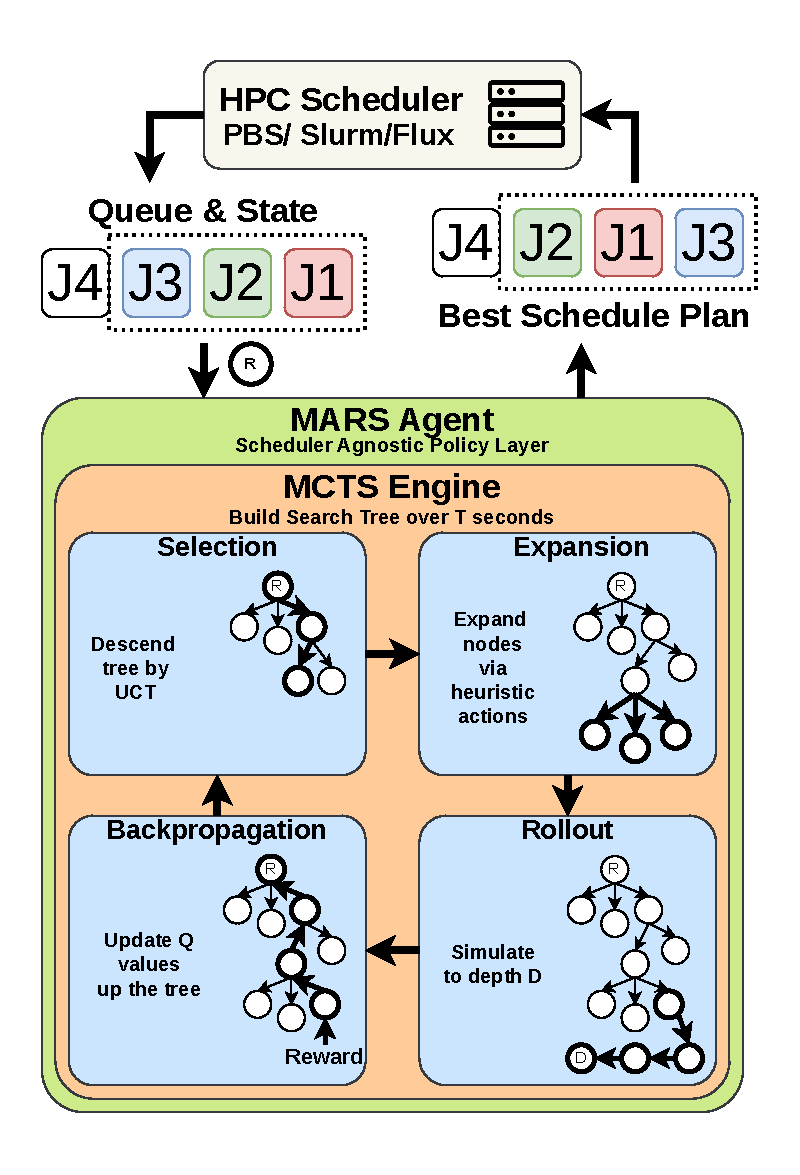
\includegraphics[width=0.68\linewidth]{figures/MCTS_overview-A.drawio-3.pdf}
  \caption{\small{MARS overview. At each scheduling cycle, the agent receives the current system state and waiting queue, and initializes the MCTS engine with a root node \protect\circled{R} representing the present state.  
  MCTS then iterates over four stages: Selection, Expansion, Rollout, and Backpropagation for a fixed budget of $T$ seconds. When the budget expires, the action leading to the most-visited child of the root is returned as the schedule plan and applied to the production scheduler by adjusting job priorities accordingly.}
%At the end, the action leading to the most visited child of the root is sent as the best schedule plan to the scheduler by tweaking the job priorities.
   }
  \label{fig:overview}
\end{figure}


\section{Background}
\textbf{Scheduling in HPC.} Scheduling in HPC systems is handled by job schedulers such as PBSPro \cite{AltairPBSPro}, Slurm \cite{SlurmDocs}, and Flux \cite{FluxFramework}. Users submit jobs using the scheduler's interface and provide the resource requirements and walltime (duration of job). In a production HPC system, the smallest schedulable unit is a node that may contain multiple CPUs and GPUs. This is because HPC centers prefer giving researchers dedicated bare metal resources to avoid interference from other users on the system. Thus, each job is characterized by the number of nodes (job size) it requires and the walltime. Scheduling in HPC is dictated by the scheduling policy, which determines the order in which the submitted jobs run on the system.

\textbf{Scheduling Policy.}  In academic work, the scheduling policy is generally viewed as the rule that determines the order in which the submitted jobs run on the system. In practice, this is much more complex. HPC facilities must perform system maintenance, meet allocation award goals of funding programs such as ALCC, INCITE, or DD \cite{allcock_expatanl_2018}, and reserve the whole or parts of the system for special requests \cite{ALCFResvPolicy, OLCFResvPolicy}. Such nuances have been ignored by the state-of-the-art scheduling, especially AI-based intelligent policies \cite{fan_deep_2021, zhang_rlscheduler_2020}. We fill in this gap by proposing MARS, which is intelligent and can easily adapt to such goals. While \S\ref{sec:related_work} expands more on prior work, Table \ref{tab:scheduling-comparison} provides an overview of the comparison.

%We extensively describe the scheduling model we use in section \ref{sec:sched_model}.

% \begin{table*}[t]
% \centering
% \begin{tabular}{ |c|c|c|c|c|  }
%  \hline
%  \multicolumn{1}{|c|}{Features} & \multicolumn{4}{|c|}{Scheduling Method} \\
%  \hline
%  & Heuristic & Optimization  & DRL\& ML & MCTS\\
%  \hline
% Requires Training & No & No & Yes & No \\
% % Easy to Configure & Yes & Yes & No & Yes \\
% Optimization goal can be changed & No & Yes & No & Yes \\
% Adapts to machine reservations & No & No & No & Yes \\
%  \hline
% \end{tabular}
% \caption{Comparison of scheduling methods.}
% \label{tab:scheduling-comparison}
% \end{table*}

\begin{table}[h]
\centering
\small % Slights reduces font size
\setlength{\tabcolsep}{3pt} % Reduces horizontal padding (default is 6pt)
\begin{tabular}{|p{3cm}|c|c|c|c|} 
 \hline
 \textbf{Features} & \textbf{Heur.} & \textbf{Opt.} & \textbf{DRL} & \textbf{MCTS} \\
 \hline
 Training Required & No & No & Yes & No \\
 \hline
 Cross System Stability & Yes & Yes & No & Yes \\
 \hline
 Goal Flexibility & No & Yes & No & Yes \\
 \hline
 Machine 
 Reservations & No & No & No & Yes \\
 \hline
 System Draining & No & No & No & Yes \\
 \hline
\end{tabular}
\caption{Comparison of scheduling methods.}
\label{tab:scheduling-comparison}
\end{table}

\begin{comment}
\textbf{Monte Carlo Tree Search}
\label{sec:mcts-background}
Monte Carlo Tree Search (MCTS) is a heuristic search algorithm for sequential decision-making that integrates classical tree search with reinforcement learning principles. The core idea is to incrementally build a search tree where nodes represent states and edges represent actions. It achieved widespread recognition through AlphaGo ~\cite{silver_mastering_2017}, which combined MCTS with deep neural networks trained via self-play to defeat the world champion in Go, a game whose state space ($\sim 10^{170}$ positions) had long been considered intractable for classical search methods such as Alpha-Beta pruning. The subsequent AlphaZero system~\cite{silver_mastering_chess_shogi_2017} generalized this approach to Chess and Shogi, demonstrating that MCTS paired with learned evaluation functions could achieve superhuman performance across multiple domains without domain-specific engineering. Crucially, AlphaZero uses MCTS in both training (to generate self-play data) and inference (to select moves), with a neural network providing value estimates and action priors that guide the search. 

In our work, we take the first steps to bring MCTS to the HPC scheduling community by relying solely on simulation rollouts for value estimation rather than neural networks, as scheduling has no notion of self-play. This also eliminates the need for training while still benefiting from the algorithm's ability to plan ahead and evaluate the long-term consequences of scheduling decisions. Figure \ref{fig:overview} provides an overview of our methodology. A chief characteristic of MCTS is that the longer it is allowed to run, the better it gets, as we show in our evaluations and also demonstrated by the AlphaZero agent \cite{silver_mastering_chess_shogi_2017}.
\end{comment}


\section{Problem Formulation}
\label{sec:problem_formulation}

We formulate HPC job scheduling as a sequential Markov Decision Process (MDP) and solve it online via Monte Carlo Tree Search (MCTS). MARS acts as a scheduler-agnostic policy layer that augments existing production schedulers with an MCTS agent, performing look-ahead planning through a discrete-event simulation (DES) of the system. 
This framework allows the agent to evaluate the long-term impacts of counterfactual actions at each decision point — without disturbing the production system. 
The remainder of this section details the DES model and its MDP formulation, then describes how MDP states are embedded within the four MCTS stages.

 

% We formulate the HPC job scheduling problem as a sequential Markov Decision Process (MDP) and solve it using Monte Carlo Tree Search (MCTS). MARS provides a scheduler-agnostic policy layer that augments existing schedulers with an MCTS agent operating exclusively on job events. 
% The agent relies on a scheduling model implemented via discrete-event simulation (DES), enabling look-ahead planning at each decision point by exploring counterfactual actions and evaluating their long-term impact on system performance.

% We first describe the scheduling model, followed by its formulation as an MDP. We then show how MDP states are embedded within MCTS as nodes in the search tree, constructed through the four canonical stages: selection, expansion, rollout, and backpropagation.

%We formulate the HPC job scheduling problem as a sequential Markov Decision Process (MDP) and solve it using Monte Carlo Tree Search (MCTS). The MCTS algorithm uses a model of the HPC system implemented using Discrete Event Simulation (DES). The simulated model is used to plan ahead at each scheduling decision by exploring various what-if actions and evaluating their long-term impact on system performance. Here, we first describe our model, followed by how the model is used to simulate a Markov Decision Process (MDP). Finally, we show how the states of the MDP can be used within the MCTS as states in the search tree built using the four stages of selection, expansion, rollout, and backpropagation.

\subsection{Scheduling Model}
\label{sec:sched_model}
The scheduling model serves two roles: it represents the states stored in the search tree, and it encodes the dynamics that govern how the system evolves when an action is applied. 

\subsubsection{Scheduling Environment} 
\label{des}

% We model the scheduling environment during search using a Discrete Event Simulation (DES) paradigm. In this paradigm, time advances discretely from one event to the next. DES has long been central to HPC scheduling research, both as a vehicle for evaluating scheduling strategies \cite{rodrigo2018scsf, dutot2017batsim, klusavcek2020alea, galleguillos2020accasim} and as a training environment for DRL-based schedulers \cite{zhang_rlscheduler_2020, fan_deep_2021, yang_deep_2022, zhang_schedinspector_2022}. 

% In this work, we consider the following event types: \lan{revised to remove CQSim as the design is general and can be applied with any simulator!}

% \begin{enumerate}
%     \item \textbf{Job Submit/Run/End}: When a jobs are submitted, run or end.
%     \item \textbf{Scheduling Cycle}: The scheduling mechanism is invoked to potentially run new jobs.
%     \item \textbf{Announce Downtime}: When the administrator announces downtime for maintenance. This is set to $48$ hours prior to when scheduled maintenance begins. From this point on, no jobs that may coincide with the maintenance shall be run.
%     \item \textbf{Scheduled Downtime Begin/End}: When scheduled maintenance begins or ends. It always begins $48$ hours from the maintenance announcement.
%     \item \textbf{Unscheduled Downtime Begin/End}: When an unscheduled/emergency maintenance begins or ends. In such a case, all running jobs are killed and returned to the queue as resubmissions.
% \end{enumerate}

% A DES simulator maintains an event queue and processes events in chronological order, each one updating the system state and potentially inserting new downstream events. Simulation begins when the first Job Submit event is processed, which in turn triggers the insertion of subsequent events such as Job Run and Job End. Every event therefore has two responsibilities when dequeued: (i) update the system state and (ii) insert any follow-on events into the queue.

% For example, a Submit event adds a job to the scheduler's waiting queue and immediately inserts a Scheduling Cycle event after it. The Scheduling Cycle event, in turn, may insert one or more Run events if new jobs can be dispatched. Each Run event inserts a corresponding End event at the appropriate timestamp based on the job's expected duration. Finally, every End event inserts another Scheduling Cycle event, since job completion frees resources and creates a fresh opportunity to dispatch waiting jobs. This loop continues until the waiting queue is empty and no further Submit events remain.

% The key insight underlying MARS is that the system state captured at each Scheduling Cycle can be cloned and replayed under different scheduling decisions, enabling the agent to evaluate the long-term consequences of alternative actions by controlling which Run events are inserted next.

% \subsubsection{The Scheduling Agent} 
% %Most HPC schedulers such as Slurm \cite{SlurmDocs} and PBSpro \cite{AltairPBSPro} are strictly FCFS and additionally employ EASY Backfilling \cite{backfill} for optimizations. 
% At each Scheduling Cycle event, the scheduler is invoked to make scheduling decisions. For a simple FCFS policy, the scheduler would go through the queue of waiting jobs one by one and run what it can until it hits a job that cannot be scheduled anymore (called the top job). This is followed by an EASY backfilling procedure that goes further down the queue, trying to schedule any jobs that won't delay the start time of the top job. Once the scheduler has a set of jobs it has determined to run, it inserts Run events for those jobs into the event queue of the simulator.

% \subsubsection{Scheduling Window} 
% Because production schedulers operate in FCFS order, optimization is typically expressed through integer priority values assigned to individual jobs \cite{allcock_expatanl_2018}. 
% This is done by implementing a window $w$ at the start of the queue of waiting jobs. The jobs that fall in this window are then ordered from high to low priority to create scheduling outcomes beyond FCFS. Once the window is shuffled, the scheduler can go over the new queue as described in the earlier section. Such a mechanism is not only used in production but also by the community in scheduling research.

We model the scheduling environment using Discrete Event Simulation (DES), in which system time advances between discrete events. This paradigm is widely used in HPC research, for strategy evaluation \cite{rodrigo2018scsf, dutot2017batsim, klusavcek2020alea, galleguillos2020accasim} and as a training environment for DRL-based models \cite{zhang_rlscheduler_2020, fan_deep_2021, yang_deep_2022, zhang_schedinspector_2022}. \emph{MARS adopts the same paradigm but uses it online}: rather than evaluating a fixed policy in simulation, the DES is invoked at every scheduling cycle as a forward model for MCTS rollouts.

The simulator processes events chronologically, with each event responsible for updating the system state and scheduling future events. We consider the following event types:

\begin{enumerate}
    \item \textit{Job Submit/Run/End}: Standard job lifecycle transitions.
    \item \textit{Scheduling Cycle}: Invokes the scheduling mechanism to dispatch jobs.
    \item \textit{Announce Downtime}: Occurs 48 hours prior to scheduled maintenance. Beyond this point, the scheduler prevents the execution of any job whose walltime overlaps with the maintenance window.
    \item \textit{Scheduled Downtime Begin/End}: Marks the start and completion of planned maintenance.
    \item \textit{Unscheduled Downtime Begin/End}: Represents emergency failures. In these instances, all running jobs are terminated and returned to the queue for resubmission.
\end{enumerate}

The simulation follows a reactive loop: a \textit{Job Submit} event triggers a \textit{Scheduling Cycle}; if resources permit, the cycle inserts \textit{Job Run} events, which in turn generate \textit{Job End} events based on the actual runtime. Every job completion (\textit{Job End}) triggers a new \textit{Scheduling Cycle} to fill the newly available resources. The core capability of MARS lies in its ability to clone the system state at any \textit{Scheduling Cycle} and replay it under alternative scheduling decisions, enabling the agent to evaluate the long-term consequences of different actions.

\subsubsection{Schedule Windowing}
At each \textit{Scheduling Cycle}, the agent determines which jobs to dispatch. While production schedulers like Slurm \cite{SlurmDocs} and PBS Pro \cite{AltairPBSPro} primarily follow First-Come-First-Served (FCFS) order, they often assign integer priority values to jobs to optimize performance \cite{allcock_expatanl_2018}. 

To simulate this, we implement \emph{a scheduling window} $w$ at the head of the waiting queue. The agent reorders the jobs within this window from highest to lowest priority according to its selected heuristic. After reordering, the scheduler processes the queue sequentially until it encounters a ``top job'' that cannot be scheduled due to resource constraints, followed by an EASY back-filling procedure that attempts to utilize remaining nodes without delaying that top job. This window-based approach allows the agent to explore scheduling outcomes beyond arrival-order FCFS.


\subsection{Markov Decision Process}
\label{sec:mdp}
The above scheduling process can be represented as a Markov Decision Process (MDP) defined by the tuple $(\mathcal{S}, \mathcal{A}, \mathcal{T}, \mathcal{R}, \gamma)$:

\begin{itemize}
    \item \textit{State} $s_t \in \mathcal{S}$: A complete snapshot of the simulator at a Scheduling Cycle event, comprising the queue of waiting jobs, the set of running jobs with their completion times, the number of available nodes, the current simulation time, and the event queue of future events. This snapshot is taken just before the scheduler has run and inserted any new Run events into the event queue.

    \item \textit{Action} $a_t \in \mathcal{A}$: A reordering of the \emph{window} which is the first $w$ jobs at the head of the queue of waiting jobs.

    \item \textit{Transition} $\mathcal{T}(s_{t+1} | s_t, a_t)$: The action reorders the first $w$ jobs in the queue, after which the scheduler runs. The transition then fast-forwards through all non-Scheduling Cycle events until the next scheduling cycle is reached.

    \item \textit{Reward} $\mathcal{R}(s_{t+1})$: An immediate reward assigned to the successor state reached after applying action $a_t$ in state $s_t$. It is computed from the set of jobs dispatched during the transition from $s_t$ to $s_{t+1}$.

    \item \textit{Discount factor} $\gamma \in [0, 1]$: The discount factor is multiplied with the reward depending on how far ahead it is in the future. A higher discount factor gives more emphasis to future rewards than the present, making MCTS less greedy.
\end{itemize}

A sequence of such states and actions forms a Markov decision process, which follows the Markov property that the future states only depend on the current state and not the history of actions and states preceding it:

\begin{equation}
    s_{\text{0}} \xrightarrow{a_0} s_1 \xrightarrow{a_1} \cdots \xrightarrow{a_k} s_{\text{k}}
\end{equation}

\subsection{Monte Carlo Tree Search (MCTS)}
\label{sec:mcts}


%The core function of MCTS is \emph{to build a search tree over action sequences, balancing exploration of untried actions with exploitation of high-reward ones.} The MDP formulation from the previous section can be utilized for this by representing each state $s_t \in \mathcal{S}$ as a node in the search tree. From each node, various actions lead to subsequent states, creating a tree-like structure

The core function of MCTS is \emph{to build a search tree that explores the space of action sequences, balancing exploration of untried actions against exploitation of high-reward ones}. The MDP formulation maps onto this tree directly: each state $s_t \in \mathcal{S}$ is represented as a node, and each action $a_t \in \mathcal{A}$ is an edge connecting a parent state to the successor state produced by the transition. Repeated application yields a tree rooted at the current system state, with each path from root to leaf representing one trajectory of look-ahead.


The algorithm is invoked at each \emph{Scheduling Cycle} event where the waiting queue contains more than one job. First, the root node of the tree is initiated using the current state of the system. Then MCTS iteratively builds a tree of system states and actions using the four stages of selection, expansion, rollout, and backpropagation. Finally, the algorithm returns the best window ordering it found from the current state, which is used by the scheduler to run new jobs. 

\subsubsection{Selection}
\label{sec:selection}
Starting from the root node, the algorithm descends the tree by selecting the child with the highest UCT score:
\begin{equation}
    \text{UCT}(s_t) = Q(s_t) + c \cdot \sqrt{\frac{2 \ln N}{n_t}}
\end{equation}
where $Q(s_t)$ is the expected reward beyond state $s_t$, $n_t$ is number of times node was visited, $N$ is the parent's visit count, and $c$ is the exploration constant. The goal of UCT is to balance exploration with exploitation of the search space. The first term is greedy in terms of selecting nodes with the highest average reward, whereas the second term grows inversely with $n_t$, promoting exploration of less visited nodes in the tree. A larger $c$ would thus promote exploration and reduce greedy behavior. The selection stage continues until it reaches a leaf of the tree. The leaf node is then passed to the next stage.

\subsubsection{Expansion}
\label{sec:expansion}
The expansion stage takes the leaf node and instantiates a child node by 
(1) copying the leaf node's simulator state, (2) reordering the queue according to the child's action, and (3) stepping the simulation forward until the next Scheduling Cycle event. This is represented by the transition $\mathcal{T}(s_{t+1} | s_t, a_{t})$. The \emph{outcome} of this action $a_{t}$ is the set of jobs $o_{t}$ that go from waiting to running, which is recorded to compute the immediate reward $\mathcal{R}(s_{t+1})$ of the node's state. When all possible actions from the leaf lead to a child node, it stops being a leaf node, and its simulator state is released from memory to conserve resources, as it won't be needed for future expansions or rollouts.

\subsubsection{Rollout}
\label{sec:rollout}
From the newly expanded leaf, the simulation is run forward with actions of random orderings of the window until termination or a predefined maximum depth for the tree is reached. The process so far can be summed up as follows:

\begin{equation}
\underbrace{s_{\text{root}} \xrightarrow{a_0} s_1 \xrightarrow{a_1} \cdots \xrightarrow{a_{k-1}} s_{\text{leaf}}}_{\text{selection}} \underbrace{\xrightarrow{a_{\text{k}}} s_{k+1}}_{\text{expansion}} \underbrace{\xrightarrow{a_{\text{rand}}} \cdots \xrightarrow{a_{\text{rand}}} s_{D}}_{\text{rollout}}
\end{equation}

where $D$ is the predefined tree depth which controls how far in the future MCTS explores.

The reward from the rollout phase is calculated by summing up the immediate rewards of state $s_{k+1}$ to state $s_{d}$ as follows:
\begin{equation}
    G_{\text{rollout}} = (1 - \gamma)\sum_{t=k+1}^{d} \gamma^{t -(k+1)} \cdot \mathcal{R}(s_t)
\end{equation}

The $(1 - \gamma)$ normalizes the reward between $[0,1]$, which is a common approach in MCTS to ensure the UCT in the selection phase is properly calibrated.

\subsubsection{Backpropagation} 
\label{sec:backpropagation}
The return $G_{rollout}$ is then propagated from the leaf back to the root. For each node $t$ representing state $s_t$, $n_t$ is incremented and the expected value $Q(s_t)$ is updated using the rollout reward and immediate reward $\mathcal{R}(s_t)$ as follows:
\begin{equation}
    Q(s_t) \gets Q(s_t) + \frac{1}{n_t} \left[ \Big( (1 - \gamma)\mathcal{R}(s_t) + \gamma \cdot G_{\text{rollout}} \Big) - Q(s_t) \right]
\end{equation}

In simple words, $Q(s_t)$ is the average rollout reward from the node $s_t$ and is used in the selection phase for the UCT equation, which guides the search.


\section{Scaling MCTS for HPC Scheduling: Challenges and Solutions}
\label{sec:implementation}

Section~\ref{sec:problem_formulation} formulated HPC scheduling as an MDP, enabling MCTS to drive what-if exploration of the scheduling process. 
In this section, we discuss the practical challenges of this approach and present solutions to address them.

\subsection{Heuristic Branching}
\label{sec:heuristic_branching}


% \begin{figure} 
%     \centering
%     \includegraphics[width=\columnwidth]{figures/polaris_window_sensitivity.png}
%     \caption{Evaluating various utility functions paired with EASY back-filling at various window sizes on a year (2024) long workload from Polaris at ALCF.}
%     \label{fig:heuristic-window-eval}
% \end{figure}

% \begin{table*}[t]
% \centering
% \begin{tabular}{llp{8cm}}
% \toprule
% \textbf{Heuristic Policy} & \textbf{Scoring Function} & \textbf{Description} \\
% \midrule
% FCFS & $s_j$ & First Come First Served. Arrival order. \\
% LCFS & $-s_j$ & Last Come First Served. Most recent first. \\
% SJF & $r_j$ & Shortest Job First. \\
% LJF & $-r_j$ & Longest Job First. \\
% SRF & $n_j$ & Smallest Resource First. Fewest nodes first. \\
% LRF & $-n_j$ & Largest Resource First. Most nodes first. \\
% SCF & $r_j \cdot n_j$ & Smallest Core/Node-Hours First. \\
% LCF & $-(r_j \cdot n_j)$ & Largest Core/Node-Hours First. \\
% FCSJ & $-w_j / r_j$ & First Come Shortest Job \\
% WFP1 & $-(w_j / r_j) \cdot n_j$ & Favors old/short jobs, avoiding large job starvation \cite{tang-cluster09}. \\
% WFP3 & $-(w_j / r_j)^3 \cdot n_j$ & Favors old/short jobs more, avoiding large job starvation \cite{tang-cluster09}. Used at ALCF \cite{allcock_expatanl_2018} \\
% FAT & $-(w_j / r_j) \cdot (n_j / N)^3$ & Favors large jobs, then old/short job \cite{tang-cluster09}. \\
% UNICEF & $-w_j / (\log_2(n_j / N) \cdot r_j)$ & Provides fast turnaround for small jobs \cite{tang-cluster09}.\\
% F1 & $\log_{10}(r_j) \cdot n_j + 870 \cdot \log_{10}(s_j)$ & Log-linear composite. Derived using Non Linear Regression \cite{f1_f4_ml}.\\
% F2 & $\sqrt{r_j} \cdot n_j + 2.56 \times 10^4 \cdot \log_{10}(s_j)$ & Square-root composite. Derived using Non Linear Regression \cite{f1_f4_ml}. \\
% F3 & $r_j \cdot n_j + 6.86 \times 10^6 \cdot \log_{10}(s_j)$ & Linear composite. Derived using Non Linear Regression \cite{f1_f4_ml}. \\
% F4 & $r_j \cdot \sqrt{n_j} + 5.30 \times 10^5 \cdot \log_{10}(s_j)$ & Mixed composite. Derived using Non Linear Regression \cite{f1_f4_ml}. \\
% \bottomrule
% \end{tabular}

% \caption{Heuristic scheduling policies. For each job $j$ in the job queue, a score is calculated using the scoring function. Then the job queue is sorted by ascending score; the lowest-scored job is at the top of the queue. The inputs to the function are: $r_j$ = walltime, $n_j$ = nodes, $N$ = system size, $s_j$ = submit time, $w_j$ = wait time.}
% \label{tab:heuristic-policies}
% \end{table*}

\begin{table}[ht]
\centering
\small
\setlength{\tabcolsep}{6pt} % Slightly more breathing room since lines are gone
\begin{tabular}{ll}
\toprule
\textbf{Heuristic Policy} & \textbf{Scoring Function} \\
\midrule
FCFS & $s_j$ \\
LCFS & $-s_j$ \\
SJF  & $r_j$ \\
LJF  & $-r_j$ \\
SRF  & $n_j$ \\
LRF  & $-n_j$ \\
SCF  & $r_j \cdot n_j$ \\
LCF  & $-(r_j \cdot n_j)$ \\
FCSJ & $-w_j / r_j$ \\
WFP1 & $-(w_j / r_j) \cdot n_j$ \\
WFP3 & $-(w_j / r_j)^3 \cdot n_j$ \\
FAT  & $-(w_j / r_j) \cdot (n_j / N)^3$ \\
UNICEF & $-w_j / (\log_2(n_j / N) \cdot r_j)$ \\
F1   & $\log_{10}(r_j) \cdot n_j + 870 \cdot \log_{10}(s_j)$ \\
F2   & $\sqrt{r_j} \cdot n_j + 2.56 \times 10^4 \cdot \log_{10}(s_j)$ \\
F3   & $r_j \cdot n_j + 6.86 \times 10^6 \cdot \log_{10}(s_j)$ \\
F4   & $r_j \cdot \sqrt{n_j} + 5.30 \times 10^5 \cdot \log_{10}(s_j)$ \\
\bottomrule
\end{tabular}
\caption{Heuristic policies and their respective scoring functions. Jobs are sorted in ascending order of scores calculated by the scoring functions with inputs: $r_j$ (walltime), $n_j$ (nodes), $s_j$ (submit time), $w_j$ (wait time), and $N$ (total system size).}
\label{tab:heuristics-policies}
\end{table}



% \begin{figure} 
%     \centering
%     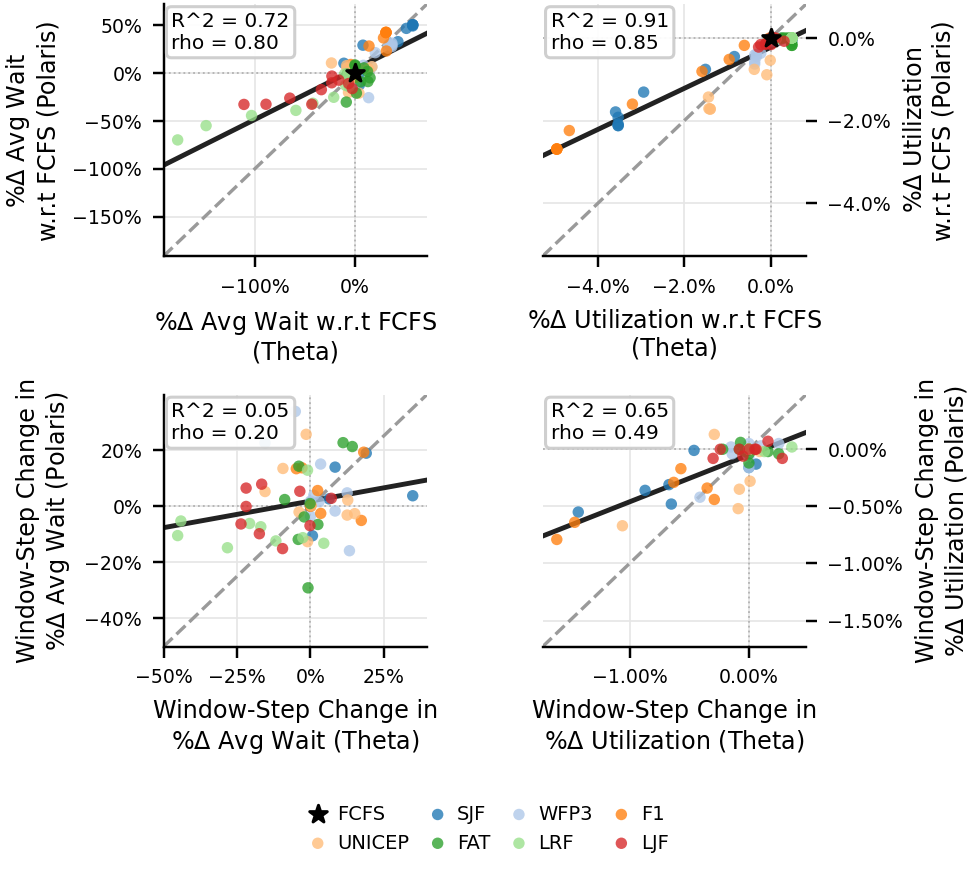
\includegraphics[width=\columnwidth]{figures/cross_system_combined_transfer.png}
%     \caption{A cross-system performance analysis of a few heuristic functions using Polaris 2024 and Theta 2021 workload. The top shows cross-system performance for (heuristic, window size) pairs relative to baseline FCFS on each system. The bottom shows the change in performance from increasing the window sizes by one step (eg: 8 $\to$ 16) normalized to FCFS baseline.}
%     \label{fig:cross-sys-w}
% \end{figure}

% We detailed that each scheduling action $a_t$ can be represented as an ordering of jobs in the window $w$ at the head of the waiting job queue. But a window of $w$ means $w!$ possible orderings of the jobs within it. This works well for window sizes up to 5, but previous studies have demonstrated a window size of $w > 20$ to show effective gains in performance \cite{fan_deep_2021, fan_scheduling_2019, zhang_rlscheduler_2020, yang-sc13}. 

% Intuitively, not all $w!$ are needed as there can be multiple window orderings that end up scheduling the same set of jobs due to resource constraints and the FCFS nature that HPC schedulers exhibit while reading the queue. In such cases, the search space is often trimmed down for MCTS using heuristics \cite{mctsjobshop}. We take a similar approach where we create multiple orderings of the queue based on the 17 heuristics listed in Table \ref{tab:heuristics-policies}. Each heuristic is unique in terms of which types of jobs it favors. The $w$ jobs at the head are then taken and ordered from low to high with respect to the scores produced by the heuristic functions. 

% The only remaining bit is to decide how many of the $w$ jobs from the head should be taken as input. Figure \ref{fig:heuristic-window-eval} shows a preliminary analysis of various heuristic functions at varying window sizes and their behavior for various metrics. All metrics were calculated by utilizing our scheduling model and simulating a year long workload from the Polaris system. The top left plot shows the overall average wait time and the top right shows the system utilization. The bottom figures are the average wait times for specific job classes Small (S) and Large (L) for the Polaris system. None of the heuristic show consistent behavior with the same window size towards the metrics. For example, the average wait under LRF increases for the small jobs where as decreases for the large. This is because systems tend to have less large jobs compared to smaller ones (Polaris had 54.1\% S and 7.5\% L jobs). Therefore no single heuristic can be perfect as there is always a dependency on the workload. In case of the Polaris and Theta systems, WFP3 seems to perform well across all except that the utilization drops. This further motivates MCTS which does only optimizes for a set metric and whose behavior does not depend on the workload.

% Branching on heuristics helps us truncate the number of possible orderings in the window, but does not help us with deciding the value of $w$. For this, we analyze a few heuristics with window sizes increasing at powers of 2 in the interval $[2,1024]$. We evaluate the heuristics for all the window sizes on year-long workloads from Polaris (2024) and Theta (2021) at ALCF \cite{ALCFData}. First, we were interested in whether the performance of the heuristics carries over from one system/workload pair to the other. Second, we wanted to see whether the effect of window size tunings also carries over from one system/workload to the other. 

% Figure \ref{fig:cross-sys-w} shows the results for our analysis. The top left panel plots the percent change in average wait, while the top right panel plots the change in utilization, with each dot representing a specific heuristic-window configuration (e.g SWF-w8, WFP3-w16, etc). Points close to the diagonal indicate similar cross-system behavior, whereas deviations from the diagonal indicate system-specific differences in effect size. The strong positive trends in both panels show that heuristics that help or hurt on Theta tend to do the same on Polaris, although the magnitude of the response is not identical across systems.

% The bottom panels of Figure \ref{fig:cross-sys-w} evaluate whether the effect of changing the heuristic window size is preserved across Theta and Polaris. Each filled dot represents one adjacent window transition within a heuristic family, such as $w=8$ to $w=16$, normalized to each system's own FCFS baseline. The bottom left panel compares the change in normalized average wait, while the bottom right panel compares the change in normalized utilization. Unlike the earlier cross-system heuristic comparison, the wait panel shows only weak agreement across systems, indicating that the effect of increasing window size is not reliably preserved. The utilization panel is more consistent, but still weaker than the direct heuristic-transfer result. This suggests that heuristic behavior is stable across systems and workloads, but the tuning of the window size is not. Furthermore, some heuristics perform well at smaller window sizes compared to their larger couterparts as seen in Figure \ref{fig:avg_wait_w}.

% We design MARS to encompass the behavior of all heuristics at all window sizes from $2-1024$ as powers of 2, which leads to a net branching factor of: $16\text{ Heuristics} \times 10 \text{ Window Sizes ($2-1024$)} + \text{ FCFS} = 161$

We define each scheduling action $a_t$ as a specific ordering of jobs within a window $w$ at the head of the waiting queue. While a window of size $w$ theoretically allows for $w!$ possible permutations, this factorial growth becomes computationally prohibitive for the $w > 20$ values typically required for significant performance gains \cite{fan_deep_2021, fan_scheduling_2019, zhang_rlscheduler_2020, yang-sc13}. However, because resource constraints and the standard First-Come-First-Served (FCFS) logic of HPC schedulers often cause different orderings to result in the same set of scheduled jobs, the search space can be effectively trimmed using heuristics. Following this intuition, we generate multiple queue orderings based on the 17 heuristics detailed in Table \ref{tab:heuristics-policies}, sorting the $w$ jobs at the head of the queue according to the scores produced by each heuristic function.

While branching on heuristics limits the number of possible orderings, it does not determine the optimal value for $w$. We analyzed window sizes increasing by powers of two in $[2, 1024]$ across year-long workloads from Polaris (2024) and Theta (2021), finding that heuristic behavior transfers reliably across systems but the optimal window size is system-dependent. To account for these system-specific variations, we designed MARS to encompass the behavior of all 16 non-FCFS heuristics across ten window sizes ($2^1$ to $2^{10}$). By integrating these combinations with the standard FCFS baseline, MARS operates with a total branching factor of:
\begin{equation}
16 \text{ Heuristics} \times 10 \text{ Window Sizes} + 1 \text{ FCFS} = 161
\end{equation}
This comprehensive action space enables the MCTS agent to dynamically adjust the trade-offs between various heuristic priorities and window depths based on the current state of the system. We employ this branching strategy for both expansions and random sampling during Rollouts.


\subsection{Tree Pruning}
\label{sec:tree_pruning}

\begin{figure} 
    \centering
    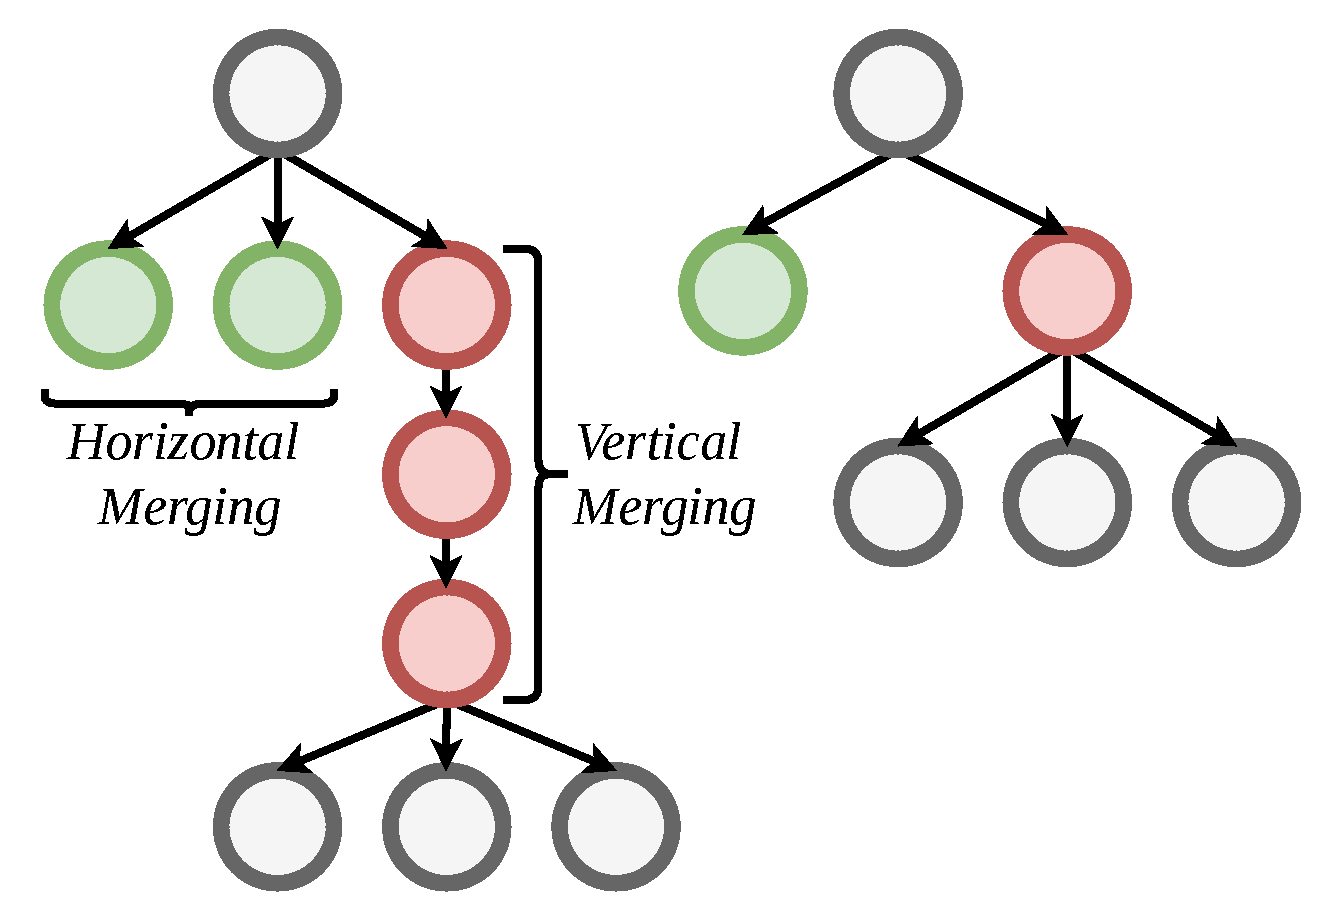
\includegraphics[width=0.6\columnwidth]{figures/Node Merging.drawio-3.pdf}
    \caption{Tree pruning via node merging. \textit{Horizontal merging} collapses sibling branches whose actions produce the same scheduling outcome; \textit{Vertical merging}  collapses consecutive scheduling cycles that yield empty outcomes (no jobs dispatched) into a single node.}
    \label{fig:node-merge}
\end{figure}

Due to resource constraints, we found that it is very common for multiple actions $a_t$ to lead to the same scheduling outcome $o_t$ or multiple scheduling cycles can produce an empty outcome $o_t$. For such instances, we merge multiple nodes into a single node as shown in Figure \ref{fig:node-merge} during the expansion stage. This provides a lower bound on the branching factor of 2. As for the depth of the tree, we manually set the maximum depth to $D$ for both expansions and rollouts. Overall, the branching factor of the tree is always between $[2,161]$ and the depth does not exceed a predefined value of $D$.


\subsection{Configurable, Training-Free Rewards}
\label{sec:rewards}

HPC scheduling metrics fall into two broad categories: \emph{system-level} and \emph{user-level}. The most widely reported metrics in each category are system utilization and average job wait time, respectively. To demonstrate MARS's reward-configurability, we introduce two reward functions, each targeting one of these metrics:

%HPC scheduling metrics fall into two categories: System Level and User Level. In each the most popular are system utilization and the wait time respectively. We introduce two rewards each optimizing for either:

\subsubsection{Cumulative Wait (CW)}: Wait time is a user-level metric, and we focus on optimizing for the average wait time $\overline{W_t}$ by keeping track of the jobs scheduled from the root node to the current state $s_t$. Then the immediate reward for the action is calculated as:

\begin{equation}
    \mathcal{R}_{\text{CW}}(s_t) = \frac{1}{1 + \overline{W_t}}
\end{equation}

\subsubsection{Cumulative Utilization (CU)}: System admins care about system utilization, which is the total useful node hours to the available node hours during system uptime. For each action, we calculate the cumulative utilization $U_t$ from the root node to the current state $s_t$ as:
\begin{equation}
    \mathcal{R}_{\text{CU}}(s_t) = U_t
\end{equation}

\subsection{Backfilling}
\begin{figure}[ht]
  \centering
  
\includegraphics[width=0.9\linewidth]{figures/backfill_fraction.png}
  \caption{\small{Fraction of dispatched jobs scheduled via EASY backfilling under representative heuristics on Theta (2021) and Polaris (2024).
Back-fill reliance varies by nearly two orders of magnitude across heuristics, demonstrating that back-filling behavior is not a fixed property of the system but a consequence of the heuristic in use.}}
  \label{fig:backfill_dist}
\end{figure}

EASY backfilling is the standard mechanism HPC schedulers use to fill resource ``holes'' and maximize system utilization. When paired with First-Come-First-Served (FCFS), it preserves fairness by forbidding any back-filled job from delaying the ``top job''---the job at the head of the queue currently blocked by resource constraints. Under heuristic-based ordering, however, the top job is no longer determined by arrival time but by the utility score in Table~\ref{tab:heuristics-policies}, which fundamentally changes which jobs back-filling protects and, consequently, how often it fires.

% Figure~\ref{fig:backfill_dist} quantifies this effect across the 2021 Theta and 2024 Polaris workloads. Back-fill share ranges from under 1\% under F1---which prioritizes large, long jobs that leave few exploitable holes---to above 95\% under WFP and LJF, which leave many small jobs available to fit into gaps. This variance shows that there is no inherent consistency in back-filling behavior across different heuristics.

Figure~\ref{fig:backfill_dist} shows back-fill shares varying from $<$1\% (F1) to over 95\% (WFP/LJF). This disparity reflects how heuristics manage candidate availability: F1 exhausts the pool by prioritizing small-footprint jobs, while SJF’s node-count indifference allows large, short jobs to head the queue. These "blockers" trap smaller jobs behind them, providing a steady supply of candidates that easily fit into back-fill windows.

%MARS therefore treats back-filling not as a post-hoc step but as part of the action's outcome.
%During MCTS simulations, the agent projects future states by applying both the selected heuristic policy and its corresponding EASY back-filling behavior simultaneously. Within our Markov Decision Process (MDP) framework, an action $a_t$ represents the selection of a specific heuristic ordering, while the resulting outcome $o_t$ is defined as the set of jobs successfully scheduled through the combination of that heuristic and its associated EASY back-filling logic.

MARS seamlessly integrates back-filling into the action outcome, rather than treating it as a secondary step. During MCTS rollouts, the agent applies a selected heuristic and its associated EASY back-filling logic in a single transition. In this MDP framework, an action $a_t$ represents the choice of a window ordering by a specific heuristic operating at a particular $w$. The outcome $o_t$ encompasses all jobs dispatched by both the primary ordering and the resulting back-fill.

\subsection{Reservations}
\begin{figure}[ht]
  \centering
  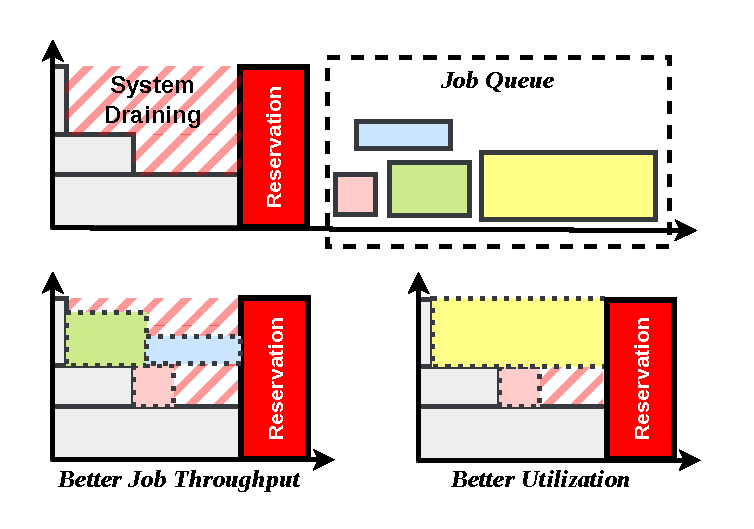
\includegraphics[width=0.8\linewidth]{figures/Reservation-F.drawio.pdf}
  \caption{\small{System-wide reservation. (Top) system state before a drain, where running jobs (left) must complete and queued jobs (right) vary in size and walltime. 
  Static heuristics commit to a fixed policy and cannot distinguish between two feasible plans: \emph{Better Job Throughput} (bottom left), which packs many small jobs to reduce wait time at the cost of fragmentation, and \emph{Better Utilization} (bottom right), which schedules a single large job aligned with the reservation boundary, sacrificing throughput. 
  MARS selects between these regimes based on the configured reward.}}
 %Reservations often lead to poor utilization because heuristics cannot pick between optimization goals. MARS must pick between better throughput (avg. wait time) or utilization.
  \label{fig:reserve_example}
\end{figure}

% Reservations are very common on HPC system, where administrators reserve a part of the system for jobs upon request \cite{ALCFResvPolicy, OLCFResvPolicy} or the whole system for maintenance. For a reservation to go into effect, the scheduler must ensure that no jobs are running during the reservation. For large system wide reservations administrators often drain the system manually by placing large jobs just before the reservations to not hurt utilization. Figure \ref{fig:reserve_example} provides an example case where the system must drain by running no jobs until the reservation goes into effect. In such cases, MARS must effectively choose between heuristics according to the optimization goal at hand. The figure shows two instances where heuristic 1 improves the throughput by packing the drain period with many small jobs compared to heuristic 2 which packs it with large jobs to improve utilization. Similar to draining, we evaluate the behavior of MARS under reservations where the primary goal is to improve the utilization of the system. For simplicity, we focus on system wide maintenance reservations in our evaluations.

System-wide reservations---used at production sites for scheduled maintenance, INCITE/ALCC awards, and specialized allocations~\cite{ALCFResvPolicy, OLCFResvPolicy}---require the scheduler to clear all active jobs before the reservation begins, forcing a system-wide drain. 
As illustrated in Figure \ref{fig:reserve_example}, MARS must schedule jobs based on the specific optimization goal during this transition. The figure highlights two distinct scenarios: The left, where throughput is improved by packing the drain period with many small jobs, and the right, which prioritizes utilization by scheduling larger requests. 

Heuristics cannot navigate this trade-off because their scoring functions are fixed and oblivious to the upcoming reservation boundary. MARS, by contrast, observes the reservation event in the simulator's event queue and shapes its scheduling decisions in the 48 hours leading up to it according to the configured reward. 
Our evaluation focuses on these system-wide maintenance reservations, assessing MARS's capacity to adaptively select heuristics that maximize system utilization leading into a reservation.

\subsection{Draining}
\begin{figure}[ht]
  \centering
  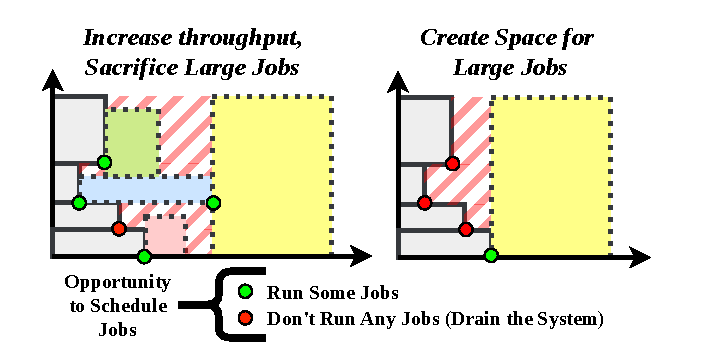
\includegraphics[width=0.8\linewidth]{figures/Drain-F.drawio.pdf}
  \caption{\small{Two schedules for the same arrival sequence. Each circle marks a scheduling cycle triggered by a job completion: green cycles dispatch new jobs, red cycles dispatch nothing (an intentional drain). \emph{Left:} dispatching small jobs whenever possible improves throughput but indefinitely delays the large yellow job, which never finds a contiguous slot. \emph{Right:} skipping three consecutive cycles deliberately holds resources idle until the fourth cycle, when enough capacity has freed up to admit the large job. }}
  %MARS must decide between increasing throughput (benefiting average wait time) or creating space for large jobs.}
  \label{fig:drain_example}
\end{figure}

% At each scheduling cycle, MARS chooses a heuristic to use by selecting the action $a_t$ that MCTS recommends. More accurately, it chooses the the outcome set $o_t$ using MCTS. In most cases multiple heuristics with their action $a_t$ will lead to the same $o_t$. Often times, it can be case that for many heuristics $o_t$ is empty. This is because heuristics block on the first job that cannot be scheduled as we saw for back-filling. MARS carefully chooses to acknowledge heuristics that don't schedule any jobs despite resource availability to schedule some jobs. Figure \ref{fig:drain_example} provides an example scenario where this may be beneficial. The figure shows some running jobs, who will trigger scheduling cycles when they finish running denoted at the filled circles. At each scheduling cycle, MARS can choose a heuristic that runs a job (green circle) or runs no jobs (red circle). On the left, if MARS were to choose heuristic 1, it schedules multiple small jobs at the cost of delaying the bigger job. On the right, if MARS chooses heuristic 2, it does not schedule any jobs for the first three cycles so that it can schedule the large job at the fourth. This is called system draining, where the scheduler holds off on scheduling any jobs to run large jobs. In our experiments we show that MARS reduces the wait times of large jobs by adaptively choosing heuristics that lead to drain cycles. 

The reservation case forces a drain because of an externally imposed deadline. MARS generalizes this idea: at any scheduling cycle, the agent can choose to drain even without an upcoming reservation, simply because doing so maximizes the configured reward over the look-ahead horizon.

At each scheduling cycle, MARS utilizes MCTS to select an outcome set ($o_t$) derived from a specific heuristic action ($a_t$). Because heuristics block on the first job that cannot be scheduled, $o_t$ may remain empty despite available resources, a state MARS leverages for ``system draining.'' Figure \ref{fig:drain_example} illustrates this process: filled circles represent scheduling cycles triggered by completing jobs, where MARS can select a heuristic that either starts a new job (green circle) or starts no jobs (red circle). The left shows a situation that schedules multiple small jobs but delays the larger request. On the right, nothing is scheduled intentionally for three cycles, allowing the large job to start at the fourth. Our experiments demonstrate that MARS effectively reduces wait times for large-scale jobs by adaptively selecting these drain-inducing heuristics. This mechanism is similar to draining for reservations except MARS can intelligently decide when to use it.

\subsection{MARS Implementation}
MARS is designed to be scheduler-agnostic, allowing it to augment existing production schedulers such as PBS or Slurm. The system is built upon the open-source discrete event simulation tool CQSim~\cite{CQSimMaster}, within which we have implemented our Monte Carlo Tree Search (MCTS) scheduling agent. CQSim has been extensively validated in prior optimization research \cite{yang-sc13, fan_scheduling_2019} and utilized in several studies involving Deep Reinforcement Learning models \cite{fan_deep_2021, li_interpretable_2023}. While the original version of CQSim is implemented in Python, we developed a C++ implementation of the architecture to fully exploit shared memory parallelism and achieve the computational speed necessary for complex search-based scheduling.


\section{Evaluation Methodology}

\subsection{Workload}

 \begin{figure} 
    \centering
    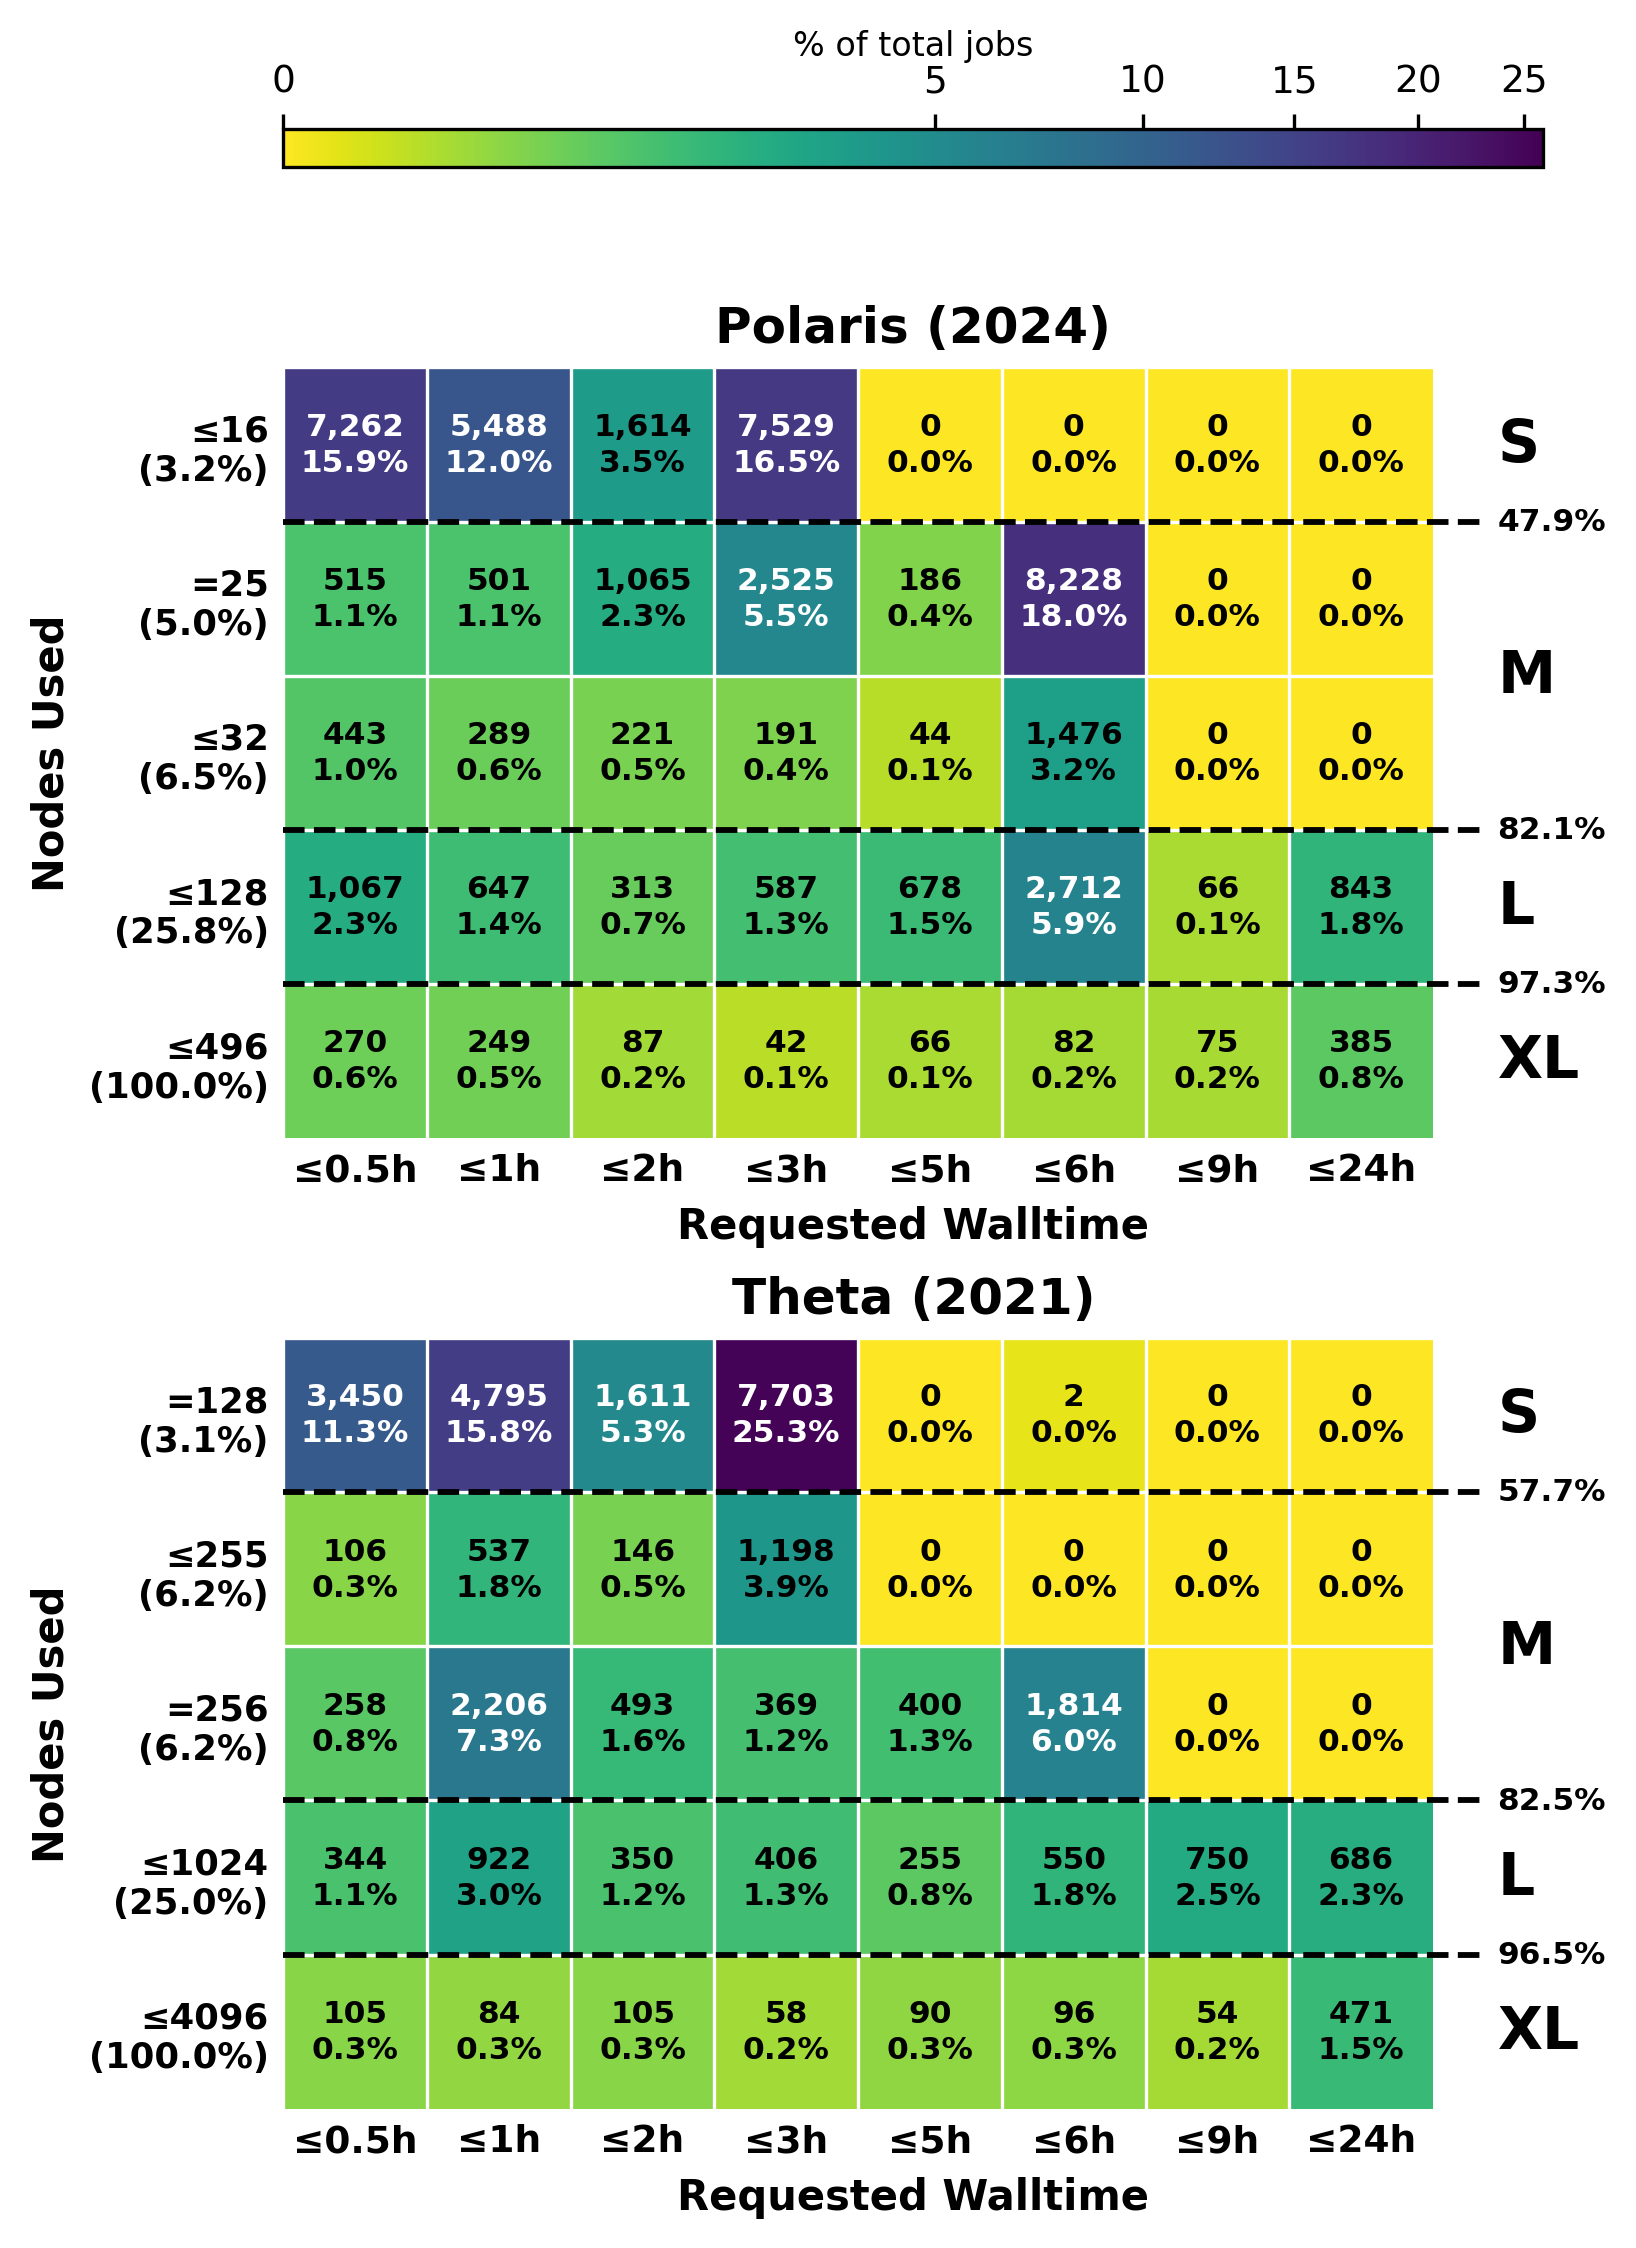
\includegraphics[width=0.8\columnwidth]{figures/heatmap_simple.png}
    \caption{Workload distribution of Polaris and Theta.}
    \label{fig:heatmap_workload}
\end{figure}

Our evaluations utilize two distinct production workloads from the Argonne Leadership Computing Facility: Theta, which includes 34,695 jobs from 2021, and Polaris, which consists of 47,183 jobs from 2024. To account for nodes dynamically reserved for debugging or special requests, we simplify the system sizes to reflect the maximum job limits allowed in the production queues, resulting in 4,096 nodes for Theta and 496 nodes for Polaris. As illustrated in Figure \ref{fig:heatmap_workload}, jobs are categorized into S, M, L, and XL sizes based on their system footprint, maintaining consistent occupancy ratios across both architectures.

Throughout the year-long data period, both systems underwent multiple scheduled and unscheduled maintenance events. We identified these downtime regions by cross-referencing job logs with the ALCF public data portal \cite{ALCFData}, allowing us to break down our analysis into specific periods of system availability. During the recorded periods, Theta experienced 28 system-wide outages, including six unscheduled emergencies, while Polaris recorded 11 outages, two of which were unscheduled.

The workload logs provide both the user-specified walltime and the requested upper bound for execution, and the recorded actual runtime. In a live environment, the true runtime remains unknown until a job completes; therefore, the MARS planning and prediction logic relies strictly on walltimes for all decision-making. To ensure our evaluations remain grounded in reality, we replay each job using its recorded actual runtime, which allows us to faithfully reproduce real-world system behavior while adhering to the information constraints present at the time of scheduling.

\subsection{Evaluation Metrics}

\begin{itemize}
    \item \textbf{Wait Time}: Wait Time is a user-level metric defined as the duration between a job's submission and its start time, which we analyze both across the total workload and categorized by specific job sizes.
    \item \textbf{System Utilization}: Measures the ratio of consumed node-hours to total available capacity during system uptime. In addition to assessing utilization for each uptime period, we specifically analyze the 48-hour windows leading up to maintenance events, as these intervals are frequently characterized by low utilization due to system draining and resource fragmentation.
    \item \textbf{Box Plot Configuration}: Both the metrics are reported using box plots where the boxes span P25--P75 with the median marked inside; whiskers extend to $\pm 1.5 \times \text{IQR}$ and the red dotted line marks the mean.
    
\end{itemize}

 \subsection{Baselines}

 \begin{figure} 
    \centering
    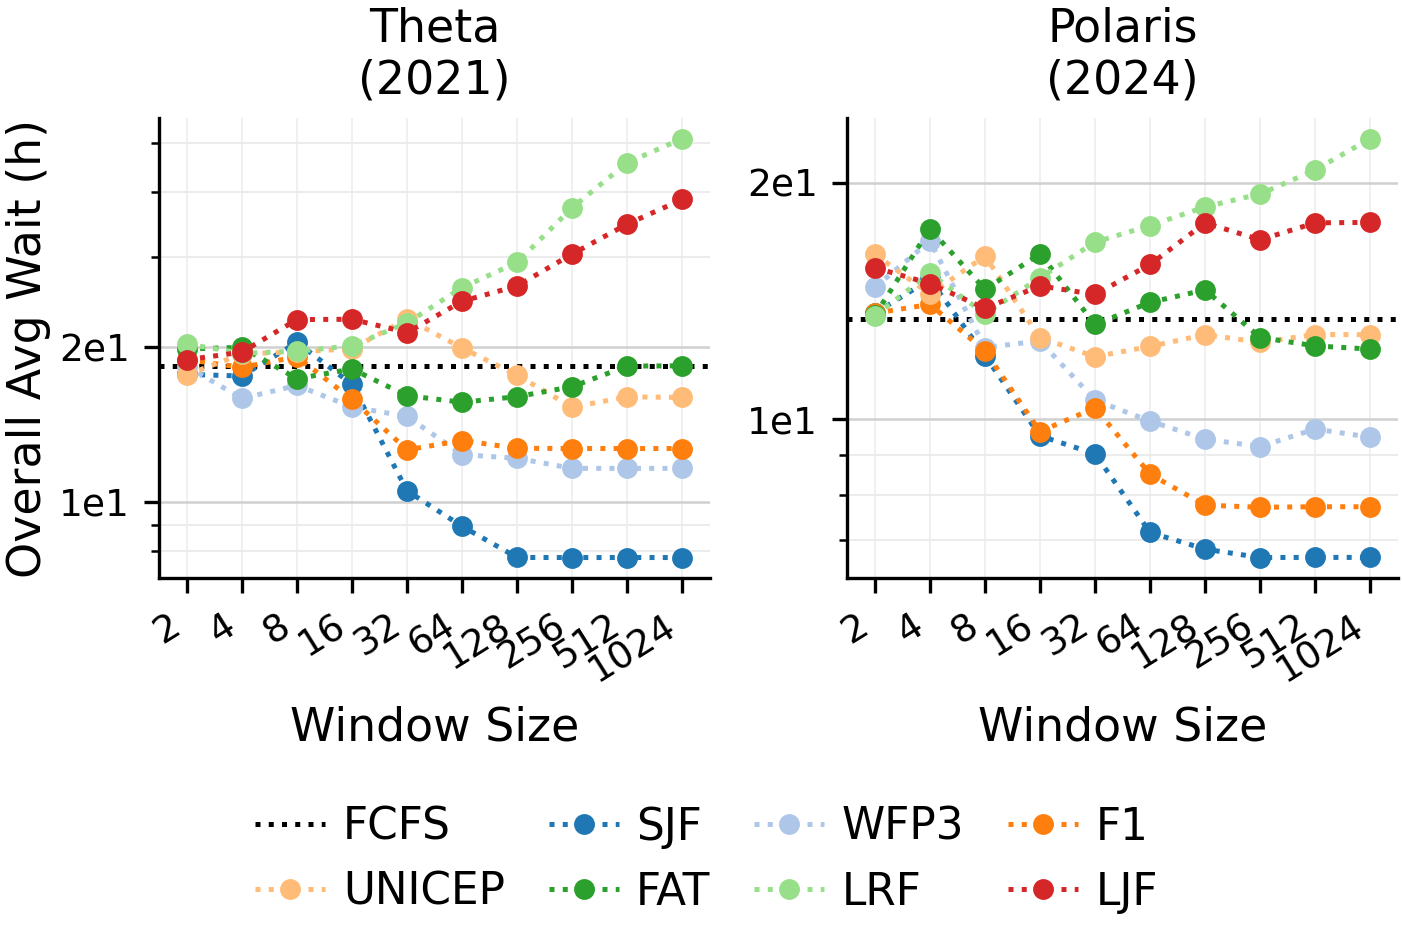
\includegraphics[width=0.8\columnwidth]{figures/avg_wait_vs_window_cross_system.png}
    \caption{Sensitivity of Average Wait Time towards window size. Baselines WFP3 and F1 reach their best performance at $w = 256$ on both. While SJF does so at $w = 1024$ on Theta.}
    \label{fig:avg_wait_w}
\end{figure}


%\begin{figure}[t]
%    \centering
%    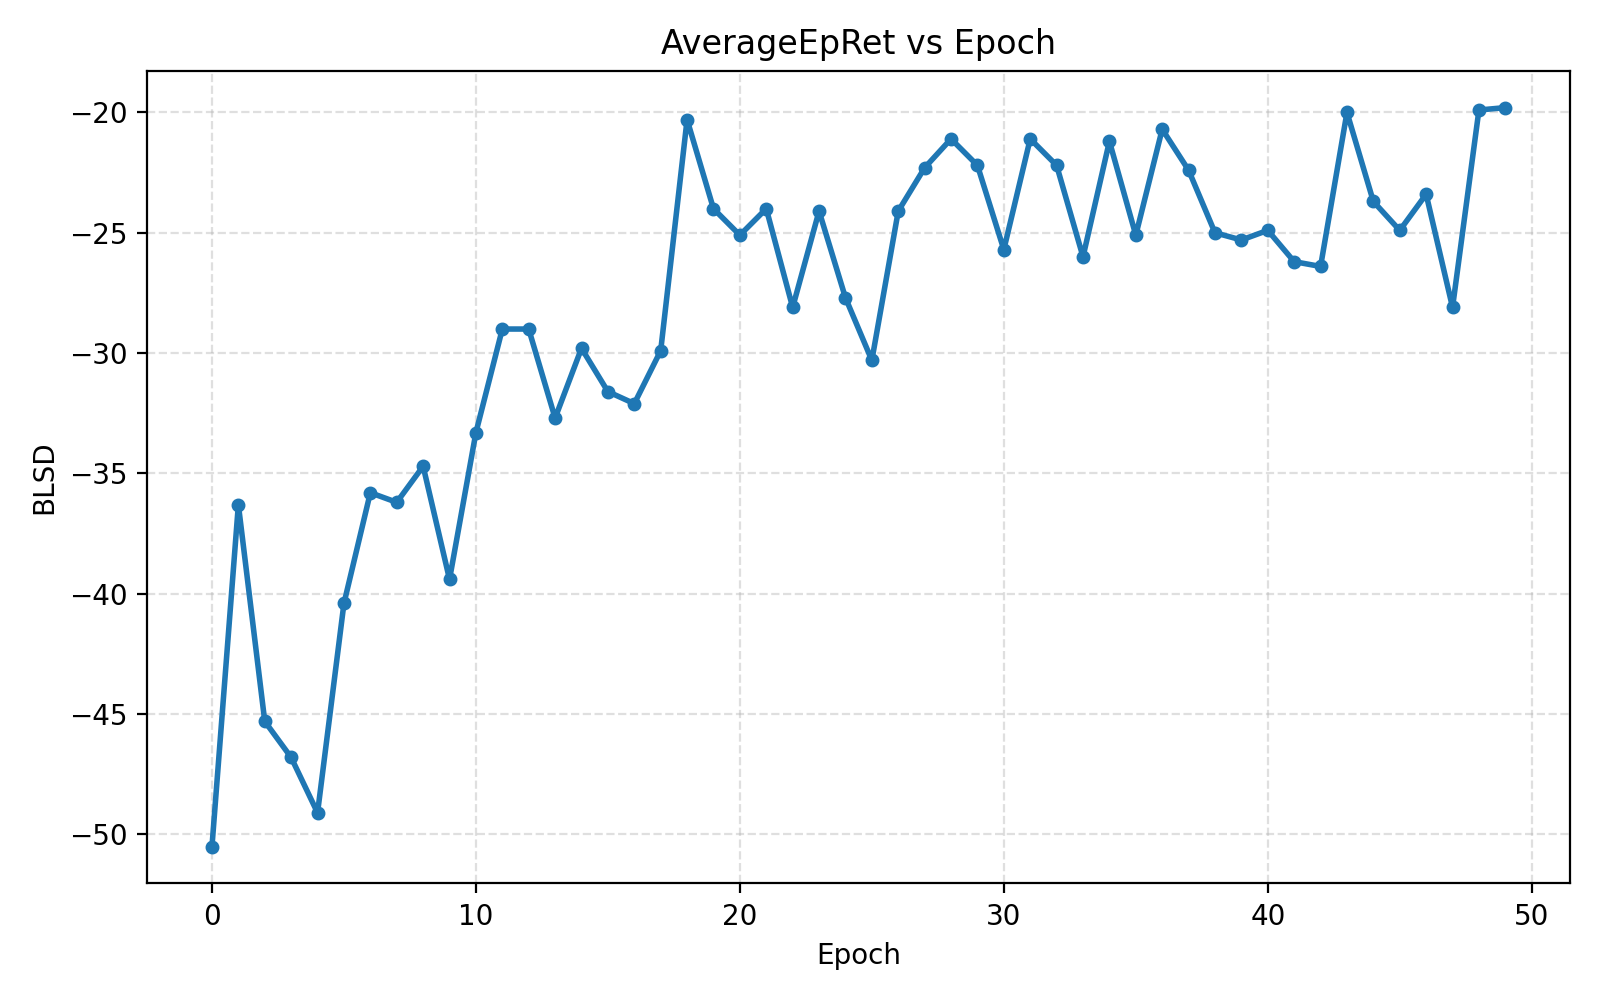
\includegraphics[width=0.6\columnwidth]{figures/theta0_gpu0.png}
%    \caption{Training curve of RLScheduler on one year of Theta workload logs (convergence within 50 epochs).}
%    \label{fig:rlsched_theta}
%\end{figure}

We compare MARS with common heuristic baselines and the state-of-the-art DRL method RLScheduler described below. The window sizes are chosen to minimize average wait time across both systems as shown in Figure \ref{fig:avg_wait_w}. Each is paired with EASY backfilling.

 \begin{itemize}
     \item \textbf{First Come First Served (FCFS)}: The most common baseline used.
     \item \textbf{Shortest Job First (SJF)}: We use a window size of $w=1024$ giving full queue visibility.
     \item \textbf{WFP}: Commonly paired with EASY backfilling at ALCF~\cite{allcock_expatanl_2018, tang-cluster09}, this heuristic scores jobs with $-(w_j^2 / r_j^3) \cdot (n_j / N)$. It favors old/short jobs while avoiding large job starvation.
     \item \textbf{F1}: To minimize average bounded slowdown, this policy utilizes the function mentioned in Table \ref{tab:heuristics-policies} derived through brute force simulation and nonlinear regression. The terms balance small, short jobs with starvation prevention for older requests, operating with a window size of 256.
     \item \textbf{RLScheduler}: The DRL scheduler~\cite{zhang_rlscheduler_2020} is retrained to minimize bounded slowdown, which jointly weighs wait time and estimated runtime and serves as the optimization target in the original paper. We train the model on one year of 2020 Theta logs and monitor convergence via episodic returns; training requires approximately 8 hours on an NVIDIA A100 40GB GPU. The retrained model is evaluated on the 2021 Theta workload. For Polaris, training on 2023 logs does not reliably converge, so we use the pre-trained model released by the original authors, justified by their reported cross-workload generalization, and evaluate it on the 2024 workload. Both evaluations use EASY backfilling. 
     %The 8-GPU-hour training cost contrasts with MARS’s training-free design, underscoring the advantage of planning-based scheduling in avoiding the data and compute burden of DRL.
     
     %The DRL-based RLScheduler \cite{zhang_rlscheduler_2020} was retrained on 2020 Theta data to minimize bounded slowdown, with convergence monitored via episodic returns (Figure \ref{fig:rlsched_theta}). We evaluated the model on 2021 Theta and 2024 Polaris workloads using EASY backfilling. 
    %\jor{The DRL-based RLScheduler \cite{zhang_rlscheduler_2020} was retrained using the 2021 Theta one-year job log with the objective of minimizing bounded slowdown. Convergence was monitored through episodic returns, as illustrated in Figure~\ref{fig:rlsched_theta}. The retrained model was subsequently evaluated on the 2021 Theta workload. For the Polaris workload, training on the 2023 Polaris job log did not converge reliably. Therefore, following the original paper's claim regarding the cross-workload generalization capability of RLScheduler, we used the released pre-trained model and evaluated it on the 2024 Polaris workload. Regarding the optimization objective, bounded slowdown was selected because it provides a more balanced and fair evaluation criterion than other candidate objectives. Specifically, it jointly considers job size, and estimated runtime. Other candidate optimization objectives include average job waiting time, job response time, and system utilization. In addition, the training process incurs substantial computational overhead; training RLScheduler on the one-year Theta workload requires approximately 8 hours on a single NVIDIA A100 40GB GPU.}
     \item \textbf{Random}: While MCTS branches on 161 policies, many result in identical outcomes (Section \ref{sec:tree_pruning}). To evaluate the reward signal's impact on search guidance, we implement a "random policy" baseline that selects a root-level branch without performing further MCTS.
    \item \textbf{MARS-CW \& MARS-CU}: Both reward configurations use a 15-second search time ($T$), consistent with standard HPC scheduling overhead constraints \cite{fan_deep_2021, fan_scheduling_2019}, and a tree depth ($D$) of 50. The exploration constant ($c$) is dynamically adjusted based on the range of $Q(s_t)$ values in the search tree, and a discount factor ($\gamma$) of 0.99 prioritizes long-term rewards. To improve performance, we use root parallelization \cite{parallel1} to construct 250 MCTS trees in parallel across 256 CPU cores within the search budget.
\end{itemize}



\section{Experimental Results}

Our evaluations are structured into three parts. First, we analyze the wait times by examining overall performance and drawing conclusions based on backfill and drain behavior. Next, we assess utilization by examining the various uptimes and utilization for the 48 hours preceding downtime to evaluate behavior before maintenance reservations. Lastly, we evaluate the performance of our MCTS algorithm using iterations achieved and the trend in the branching factor. The results reveal two key properties of MARS: its ability to adapt search behavior to the configured reward without retraining, and its responsiveness to live system state within each 15-second scheduling cycle, proactively shaping the schedule rather than relying on backfill to create opportunities.

%The results for our evaluations are structured into four parts. First we look at the overall performance during the years using wait time and utilization during up times. Then specifically for MARS-CU we further look at the utilization 48 hours prior to downtime to view its performance before maintenance reservations. Then we look at MARS-CW's performance for wait time broken down by job size and show that it is able to create holes in the schedule by draining the system when needed to reach its optimization goal. Across all four parts, results illustrate MARS's two core properties: the search adapts its behavior to the configured reward without retraining, and it does so by responding to the live system state within each 15-second scheduling cycle — proactively creating scheduling holes rather than waiting for backfill to find them.

\subsection{Job Wait Time}
\label{sec:wait_time}

\begin{figure}[t]
    \centering
    
\includegraphics[width=0.8\linewidth]{figures/wait_boxplot.png}
    \caption{\small{Wait time distribution on Theta and Polaris. MARS-CW reduces P75 wait time by 64\% on Theta and 43\% on Polaris relative to WFP (production baseline).}}
    \label{fig:overall_wait}
\end{figure}


\subsubsection{Overall Performance}
Figure~\ref{fig:overall_wait} compares the overall wait time distribution across baselines and MARS configurations. Three primary trends emerge. First, RLScheduler exhibits the highest wait times on both systems, underperforming every heuristic and even the Random baseline; this is consistent with the convergence and generalization issues reported for pure DRL schedulers \cite{zhang_rlscheduler_2020}. Second, MARS-CW, which optimizes directly for wait time, achieves the lowest median and 75th-percentile wait times on both systems, with tail behavior comparable to the strongest heuristic baselines. Third, while SJF and F1 outperform the production baseline (WFP) on wait time, they are not used in production because they sacrifice system utilization, a trade-off quantified in Figure~\ref{fig:overall_util}.

% Figure~\ref{fig:overall_wait} compares the overall wait time distribution across baselines and MARS configurations. Three observations stand out. First, RLScheduler exhibits the highest wait times on both systems; worse than every heuristic and even the Random baseline and consistent with the convergence and cross-system generalization issues reported for DRL schedulers \cite{zhang_rlscheduler_2020}. Second, MARS-CW, which optimizes directly for wait time, achieves the lowest median and P75 wait times on both systems, with tail behavior comparable to the strongest heuristic baselines (analyzed further by job size in Section~\ref{sec:results-drainbf}). Third, SJF and F1 outperform WFP on wait time but are not used in production because they sacrifice system utilization; a trade-off we quantify next in Figure~\ref{fig:overall_util}.

\subsubsection{Performance by Job Size}
\label{sec:results-jobsize}

\begin{figure*}[htbp]
  \centering
  
\includegraphics[width=0.8\linewidth]{figures/wait_by_group.png}
  \caption{\small{Wait Time distributions on Theta and Polaris broken by job size. Compared to production baseline WFP, MARS-CW performs 43.10\% and 33.40\% better on the mean for S and M jobs on Theta. Similarly, 20.94\% and 21.67\% better on the mean for Polaris. For the large jobs significant improvements are seen at P50. 60.38\% for L and 61.83\% for XL on Theta. For Polaris, 34.69\% for L and 21.62\% for XL.}}
  \label{fig:job_wise_wait}
\end{figure*}
Figure \ref{fig:job_wise_wait} provides a breakdown of wait times based on job scale. The DRL baseline shows little sensitivity to job size, except for XL jobs on Polaris. In contrast, MARS-CW yields substantial median improvements for large jobs. While tail behavior for larger jobs may appear higher, this is a byproduct of the reward function focusing on average wait time to maximize overall system responsiveness. The Random baseline serves as a competitive upper bound for heuristic branching, yet MARS consistently outperforms it by successfully guiding the search toward specific wait time or utilization objectives, as detailed in Section \S\ref{sec:util}.

% Figure \ref{fig:job_wise_wait} provides a breakdown of wait times for both systems based on job size. The DRL method does not show preference to job sizes except for XL jobs on Polaris workload. While the tail behavior of MARS-CU seems worse, this is only because it only makes significant improvements within P50 for the larger jobs. We explain why it looses out at the tail on the next section. Random performs competitively among the job classes, providing an upper bound to heuristic branching gains on wait time. But it also shows that MARS is able to guide the search with it reward towards wait time or utilization as we will see in section \S\ref{sec:util}.

\subsubsection{Draining \& Backfill Dynamics}
\label{sec:results-drainbf}

\begin{figure}[htbp]
    \centering
    
\includegraphics[width=\columnwidth]{figures/drain_overview_all_except_rlscheduler.png}
    \caption{\small{Percentage of jobs scheduled using backfill for heuristics or draining for MARS. The left shows the overall across all jobs, the right breaks down by job class.}}
    \label{fig:drain_dist}
\end{figure}


 \begin{figure}[h]
    \centering
    
\includegraphics[width=0.8\columnwidth]{figures/drain_sequence_combos.png}
    \caption{\small{Percentage of various job sequences scheduled by MARS after draining. The sequences are created using job classes and look at the first three jobs scheduled post-drain. (*) indicates any job class S/M/L/XL. Theta has a majority of S jobs, while Polaris has M jobs.}}
    \label{fig:drain_seq}
\end{figure}

 \begin{figure}[h]
    \centering
    
\includegraphics[width=\columnwidth]{figures/backfill_drain_grid_combined.png}
    \caption{\small{Stacked histograms of the wait times broken by Drain and Backfill jobs. A thicker distribution to the left indicates better performance. MARS-CW clearly outperforms WFP in S/M/L but suffers at tail of XL as those jobs are not scheduled using drain on Theta.}}
    \label{fig:drain_backfill_dist}
\end{figure}

To explain these performance shifts, Figure \ref{fig:drain_dist} contrasts heuristic backfilling with MARS draining strategies. MARS-CW drains significantly more frequently than MARS-CU, as utilization-based rewards discourage leaving nodes idle. While heuristic backfilling becomes less effective as jobs scale from S to XL, MARS-CW uses draining to schedule the majority of L and XL jobs. However, Figure \ref{fig:drain_backfill_dist} also reveals weaker tail performance for these large classes because the reward prioritizes average wait time. This objective favors global throughput by scheduling the more prevalent S and M jobs immediately after a drain. As shown in Figure \ref{fig:drain_seq}, MARS-CW frequently schedules sequences such as S-S-* or M-M-* after a drain event, reflecting the fact that S jobs dominate the Theta workload and M jobs dominate the Polaris workload.


% Figure \ref{fig:drain_dist} provides an overview of how heuristics and MARS utilize backfilling or draining strategies, both overall and per job class. Three key observations emerge: (1) MARS-CW drains significantly more frequently than MARS-CU, which aligns with the expectation based on the differing rewards. A utilization-based reward system would not encourage draining the system. (2) The trend for using backfilling decreases from S to XL for heuristics, suggesting that backfill struggles to identify suitable holes for the larger jobs. (3) MARS-CW employs draining to schedule the majority of the L and XL jobs on Theta and XL jobs on Polaris. We further analyze the job distributions in Figure \ref{fig:drain_backfill_dist}, where we observe a decline in tail performance for both L and XL jobs. This is because MAR-CW refrains from draining for these jobs. This decision stems from a reward system that prioritizes average wait time, which ultimately favors overall throughput and schedules more prevalent S and M jobs, as depicted in Figure \ref{fig:drain_seq}. The figure confirms that MARS-CW tends to schedule multiple S or M jobs consecutively after draining in many instances. The tail behavior of MARS-CW is largely related to how it drains and makes space for the large jobs. We observe S-S-* and M-M-* sequences as frequently as L-*-* sequences on Theta and Polaris, respectively. This is because S jobs are the majority in Theta workload and M jobs on Polaris.

\subsection{System Utilization}
\label{sec:util}

\begin{figure}[htbp]
    \centering
    
\includegraphics[width=0.8\linewidth]{figures/util_uptime.png}
    \caption{\small{Utilization distributions for the system uptimes. RLScheduler reports overall utilization the for year as it does not model downtimes.}}
    \label{fig:overall_util}
\end{figure}

\begin{figure}[htbp]
  \centering
  
\includegraphics[width=0.8\linewidth]{figures/util_drain_2day.png}
  \caption{\small{Utilization distributions for 48 hours prior to all scheduled down times. Theta had 21 down times in 2021 and Polaris had 9 in 2024.}}
  \label{fig:drain_util}
\end{figure}


Figure \ref{fig:overall_util} illustrates the overall utilization for different uptime windows. MARS-CU performs exceptionally well on the Theta workload and slightly better on the Polaris workload. For RLScheduler, we report the utilization as a whole year since it lacks model downtimes. As mentioned in the previous section, MARS-CU effectively prevents system draining, thereby increasing its utilization. However, MARS-CW, F1, and SJF ultimately suffer due to the trade-off between optimizing for wait time and utilization. Specifically, MARS-CW loses out on utilization because of system draining.

Figure \ref{fig:drain_util} illustrates utilization over the 48 hours preceding scheduled downtime for both systems. On Theta, MARS-CU consistently outperforms the other methods across all utilization metrics. In contrast, Polaris exhibits minimal variance in utilization due to the nature of its workload: there are not enough jobs to fill the system’s capacity on the day before downtime. However, the heuristic baselines specifically show substantial variance before downtime on Theta, indicating instability in meeting utilization goals. MARS-CU, by contrast, maintains a more stable utilization level on Theta and achieves the utilization target in most cases.



\subsection{MCTS \& Simulation Performance}
\label{sec:mcts_runtime}

\begin{figure}[t]
  \centering
  
\includegraphics[width=\linewidth]{figures/mcts_iterations_branching_div250.png}
  \caption{\small{Box plots for the single core iterations achieved by MCTS in 15 s (left) and the branching factor at the root of the tree after pruning (right) for the whole log.}}
  \label{fig:mcts_perf}
\end{figure}

A single Monte Carlo Tree Search (MCTS) comprises the four stages we discussed at the paper’s outset. The number of iterations it can execute is often used as a metric to assess the performance of the MCTS implementation. Figure~\ref{fig:mcts_perf} illustrates the runtime behavior of MCTS across the two systems. The left graph shows the distribution of MCTS iterations completed per scheduling cycle within the 15-second time limit for a single tree (single core) on average. Both MARS-CW and MARS-CU achieve hundreds of iterations on a single core, demonstrating that the C++ parallel implementation provides sufficient search depth for meaningful look-ahead on production workloads. The right graph presents the distribution of the observed branching factors. Despite a theoretical maximum of 161 branches, the effective branching factor is significantly lower for most cycles. This suggests that resource constraints and identical heuristic orderings frequently collapse the action space. Additionally, the two MARS configurations exhibit similar branching distributions, indicating that the reward signal influences which branch is selected rather than how many branches are available.



\section{Related Work}
\label{sec:related_work}
% \paragraph{Heuristics}
% The most prevalent scheduling approach in production HPC systems relies on heuristic functions. A simple example is First Come First Served (FCFS). More sophisticated utility-based approaches assign priority scores to jobs calculated by functions whose inputs combine attributes such as wait time, walltime, and job size. Utility functions have been a common method used on production systems at Argonne Leadership Computing Facility \cite{allcock_expatanl_2018, tang-cluster09}. While these policies are transparent and easy to configure, their core limitation is that they \emph{promote or demote} specific jobs based on fixed scoring rules rather than directly optimizing for system-level metrics such as average wait time, bounded slowdown, or utilization. As a result, their performance is highly sensitive to workload characteristics, and no single heuristic consistently optimizes common scheduling objectives across diverse workloads, as we also show in this work.

% \paragraph{DRL} The first study that went beyond heuristic utility methods used a Machine Learning (ML) approach where a set of utility functions was calculated using non-linear regression \cite{f1_f4_ml}. Deep Reinforcement Learning (RL) methods have also been developed to have better performance than common utility functions \cite{fan_deep_2021, zhang_rlscheduler_2020}. Both these methods are highly dependent on historical data and training. Furthermore, optimization goals cannot be changed without retraining, and cross-system performance is not optimal \cite{zhang_rlscheduler_2020}

% \paragraph{Specialized Optimization}
% A third category employs optimization techniques that are able to incorporate various optimization objectives, but do not optimize for common systems metrics such as wait time, slowdown, or utilization. Instead, their optimization goals are tuned for specific scenarios like adapting to changing electricity prices \cite{yang-sc13} or maximizing burst buffer utilization \cite{fan_scheduling_2019}.

\paragraph{Heuristics}
The most prevalent scheduling approach in production systems relies on heuristic functions, such as First-Come-First-Served (FCFS) or sophisticated utility-based scoring \cite{backfill,allcock_expatanl_2018, tang-cluster09,alcfAuroraRunningJobs,nerscQueuesChargesPolicy}. These methods are transparent and do not require training, offering high stability across different scenarios. However, as noted in Table~\ref{tab:scheduling-comparison}, they lack the flexibility to adapt to changing optimization goals or complex constraints like machine reservations, as their scoring rules are rigid and myopic, not considering future states of the machine.

\paragraph{Deep Reinforcement Learning (DRL)} 
To improve upon static heuristics, DRL methods based on deep neural networks have been developed to learn scheduling policies through experience \cite{fan_deep_2021, zhang_rlscheduler_2020}. While they can outperform heuristics, they require extensive training and are highly sensitive to workload distributions. Furthermore, DRL approaches lack goal flexibility: changing optimization objectives typically requires retraining. They also struggle with cross-machine stability, as a policy trained on one system's workload often performs poorly when deployed on another with different characteristics \cite{zhang_rlscheduler_2020}.

\paragraph{Specialized Optimization}
This class of methods applies mathematical optimization techniques to address specific scenarios, such as adapting to shifting electricity prices \cite{yang-sc13} or maximizing burst buffer utilization \cite{fan_scheduling_2019}. These approaches support flexible objective design and do not require training, offering strong stability across systems.  However, they typically lack native support for dynamic machine reservations, which often requires additional mechanisms to incorporate look-ahead reasoning.


\paragraph{Innovation}
MCTS has been explored for combinatorial planning problems such as job shop scheduling \cite{jssp1, jssp2} and constrained staff scheduling \cite{staffsched}, where the underlying problems are NP-hard. 
In contrast, this work is \emph{the first to use MCTS as a training-free, goal-configurable alternative to DRL for HPC scheduling}. 
Unlike DRL-based schedulers, which require extensive offline training and retraining when objectives change, our approach operates without any prior training and directly adapts to configurable goals at inference time. 
As shown in Table~\ref{tab:scheduling-comparison}, MCTS naturally handles machine reservations through explicit simulation of future scheduling states. It further provides high goal flexibility, allowing objectives such as wait time or utilization to be swapped without architectural modifications or expensive retraining.


%Our adaption is the first for HPC batch scheduling which represents a versatile alternative that combines the strengths of optimization and search without the need for prior training. As shown in Table~\ref{tab:scheduling-comparison}, MCTS is uniquely capable of adapting to machine reservations by simulating future scheduling states. It offers high goal flexibility—allowing objectives like wait time or utilization to be swapped without architectural changes—while maintaining stability across different machine configurations because it does not rely on system-specific historical training data.

% \section{Discussion}

% \subsection{Rapid Convergence and Flexibility}
% Unlike DRL methods, which often struggle with convergence and rigidity in HPC environments \cite{fan_deep_2021, zhang_rlscheduler_2020}, MARS utilizes MCTS to achieve convergence within seconds. By bypassing lengthy training phases, MARS scales its search performance directly through increased iteration counts or parallel tree aggregation, providing a more responsive framework for real-time scheduling.

% \subsection{Proactive Draining vs. Reactive Back-filling}
% Traditional scheduling relies on pairing heuristics with back-filling to improve utilization. However, in intelligent scheduling, back-filling becomes inconsistent because its effectiveness depends on which job the specific heuristic blocks (Figure \ref{fig:backfill_dist}). MARS shifts the focus from waiting for resource ``holes'' to proactively creating them through system draining. This approach generalizes across various heuristics and avoids the limitations of heuristic-dependent back-fill utilization.

% \subsection{Training-Free Reward Configuration}
% MARS demonstrates that optimization goals can be met through easily configurable rewards without the need for model training. This allows the search process to be dynamically guided toward specific metrics, providing more consistent optimization than static heuristics, which often favor one metric at the expense of others.

% \subsection{Robustness to Model Complexity}
% While MARS requires a simulation model, its core mechanism—queue reordering—remains effective regardless of the model's complexity. We demonstrate this by successfully integrating uptime and downtime logic into the simulation framework. This suggests that the MCTS-based search space remains stable and functional even as the underlying system model incorporates more sophisticated real-world constraints.

\section{Conclusion}
%We presented MARS, an MCTS-based HPC scheduler that requires no training and whose optimization goal is configurable through a reward function — the MCTS search then adapts its decisions to that goal by responding to the live system state within a 15-second budget. Unlike DRL methods that struggle with convergence and cross-system generalization~\cite{fan_deep_2021, zhang_rlscheduler_2020}, MARS converges within seconds and scales through parallel tree construction.
%Our two reward formulations, Cumulative Wait (MARS-CW) and Cumulative Utilization (MARS-CU), demonstrate that optimization goals can be met without model training, providing more consistent metric-specific optimization than static heuristics which inevitably trade one metric for another.
%Rather than relying on back-filling to fill resource holes reactively, MARS proactively drains the system to schedule jobs, especially for reducing wait times of larger jobs on both Theta and Polaris.
%By integrating uptime and downtime logic directly into the simulation, MARS remains stable and functional under real-world constraints, demonstrating that queue reordering via MCTS generalizes beyond simple workload replay.

We presented MARS, an MCTS-based HPC scheduler that requires no training and whose optimization goal is configurable through a reward function. At each scheduling cycle, the MCTS search adapts its decisions to the configured goal by responding to the live system state within a scheduling budget. Unlike DRL methods that require hours of training and generalize poorly across systems, MARS produces actionable decisions in seconds and scales through parallel tree construction. 
In this study, the two reward formulations demonstrate that optimization goals can be met without model training, providing more consistent metric-specific optimization than static heuristics, which inevitably trade one metric for another.
Rather than relying on back-filling to fill resource holes reactively, MARS proactively drains the system to admit large jobs, reducing wait times for larger jobs on both Theta and Polaris. 
By incorporating uptime and downtime logic, MARS remains stable under realistic constraints like scheduled maintenance and emergency outages, demonstrating that MCTS-driven queue reordering generalizes effectively beyond simple workload replay.

% Future work involves several key areas. Firstly, Random performs exceptionally close to MARS, suggesting that further optimizations can only be achieved beyond heuristic branching. Secondly, simulating back-filling is computationally expensive. Moving beyond heuristic branching will unveil additional optimizations and enhance performance in terms of the number of iterations performed. Thirdly, a sensitivity study is planned to examine how MARS is influenced by tree depths ($\gamma$), parallelization, and search time. Lastly, adapting to more intricate models of high-performance computing (HPC) systems, including topology and workflow scheduling, is a priority.

Future work will move beyond heuristic branching to surpass its current performance limits and reduce the computational overhead of simulating back-filling. We plan sensitivity studies on tree depth, $\gamma$, parallelization, and search time, while extending MARS to handle more complex features such as topology and workflow scheduling. It is also worth investigating various reward schemes per job group and incentives that could increase draining for specific jobs.

We will release MARS, along with the associated datasets and scheduling simulator, as open source on GitHub to support reproducibility and foster collaboration within the community.


%\section{Future Work}






% trigger a \newpage just before the given reference
% number - used to balance the columns on the last page
% adjust value as needed - may need to be readjusted if
% the document is modified later
%\IEEEtriggeratref{8}
% The "triggered" command can be changed if desired:
%\IEEEtriggercmd{\enlargethispage{-5in}}

% references section

% can use a bibliography generated by BibTeX as a .bbl file
% BibTeX documentation can be easily obtained at:
% http://mirror.ctan.org/biblio/bibtex/contrib/doc/
% The IEEEtran BibTeX style support page is at:
% http://www.michaelshell.org/tex/ieeetran/bibtex/
%\bibliographystyle{IEEEtran}
% argument is your BibTeX string definitions and bibliography database(s)
%\bibliography{IEEEabrv,../bib/paper}
%
% <OR> manually copy in the resultant .bbl file
% set second argument of \begin to the number of references
% (used to reserve space for the reference number labels box)
% \begin{thebibliography}{1}

% \bibitem{IEEEhowto:kopka}
% H.~Kopka and P.~W. Daly, \emph{A Guide to \LaTeX}, 3rd~ed.\hskip 1em plus
%   0.5em minus 0.4em\relax Harlow, England: Addison-Wesley, 1999.

% \end{thebibliography}
\bibliographystyle{IEEEtran}
\bibliography{IEEEabrv,references}




% that's all folks
\end{document}


